\documentclass[german]{spicker}
\usepackage{textcomp}
\usepackage{forest}
\usepackage{wasysym}

%\addbibresource{para.bib}

\title{Parallele Rechnerarchitekturen}
\subtitle{Sommersemester 2023}
\university{Fachhochschule Aachen}
\programme{Angewandte Mathematik und Informatik, M. Sc.}
\lecturer{Dr. Marcus Richter, Jochen Kreutz}

\author{Patrick Gustav Blaneck, Sven Bergmann}

\makeindex[intoc]
\makeindex[intoc, name=Beispiele,title=Beispiele]
\makeindex[intoc, name=Aufgaben,title=Aufgaben]


% Setup for SI units
\sisetup{
  per-mode=fraction,
  fraction-function=\tfrac
}
\DeclareSIUnit{\flops}{FLOPS}
\DeclareSIUnit{\cores}{cores}
\DeclareSIUnit{\cycle}{cycle}
\DeclareSIUnit{\cycles}{cycles}

% Forschungszentrum Jülich color
\definecolor{fzj}{rgb}{0, 0.24, 0.42}


\newenvironment{jsc}[2][\empty]{%
\ifx\empty#1
\index[Beispiele]{#2}%
\else
\index[Beispiele]{#1!#2}%
\fi
\label{jsc:#2}%
\begin{tcolorbox}[%
        colbacktitle=fzj!75!black,
        colback=fzj!5!white,%
        colframe=fzj!75!black,%
        base={#2},%
        label={%
                \ifx\empty#1
                {jsc:#2}%
                \else
                {jsc:#1:#2}
                \fi
            },
        % before title={%
        %         {\usekomafont{spickerboxtype}{Definition:}\hspace*{5mm}}
        %     },
        title={%
                \vphantom{Hy}%
                \usekomafont{spickerboxtitle}{{#2}}%
                \ifx\empty#1
                {}
                \else
                {
                    \hspace{2.5mm}\usekomafont{spickerboxsubtitle}{#1}
                }
                \fi
            },
        after title={%
                {\hfill\usekomafont{spickerboxtype}{Jülich Supercomputing Centre}}
            },
        % after title={
        %         {\usekomafont{spickerboxsubtitle}{
        %                     \ifx\empty#1
        %                     {\hfill}
        %                     \else
        %                     {\hfill #1}
        %                     \fi
        %                 }}
        %     },
    ]%
    }%
    {%

\end{tcolorbox}}


\newenvironment{aufgabe}[2][\empty]{
\ifx\empty#1
\index[Aufgaben]{#2}
\else
\index[Aufgaben]{#1!#2}
\fi
\label{Aufgabe:#2}
\begin{tcolorbox}[
  skin=bicolor,
  colbacktitle=fhmint!75!black,
  colback=fhmint!5!white,
  colbacklower=fhmint!50!black,
  colframe=fhmint!75!black,
  base={#2},
  label={
          \ifx\empty#1
          {Aufgabe:#2}
          \else
          {Aufgabe:#1:#2}
          \fi
      },
  title={
          \vphantom{Hy}
          \usekomafont{spickerboxtitle}{{#2}}
          \ifx\empty#1
          {}
          \else
          {
              \hspace{2.5mm}\usekomafont{spickerboxsubtitle}{#1}
          }
          \fi
      },
  after title={
          {\hfill\usekomafont{spickerboxtype}{Aufgabe}}
      },
    ]
    }
    {
\end{tcolorbox}}

\begin{document}
\maketitle
\tableofcontents
\disclaimer

\section{Rechnerarchitekturen}\label{sec:rechnerarchitekturen}

\subsection{Einführung}\label{subsec:einfuehrung}

\begin{defi}{Struktur}
    Unter der \emph{Struktur} einer Rechnerarchitektur versteht man die Art der Verknüpfung der verschiedenen Hardwarekomponenten eines Rechner miteinander.
    
    Sie ist in der Regel \emph{statisch}.
\end{defi}

\begin{defi}{Organisation}
    Die \emph{Organisation} einer Rechnerarchitektur steht für die zeitabhängigen Wechselwirkungen zwischen Komponenten und die Steuerung dieser Komponenten.
    
    Diese Wechselwirkungen können \emph{dynamisch} sein.
\end{defi}

\begin{defi}{Implementierung}
    Die \emph{Implementierung} einer Rechnerarchitektur bezeichnet die Ausgestaltung einzelner Bausteine.
    
    Sie gibt die \emph{Größe} eines Systems an.
\end{defi}

\begin{defi}{Leistung}
    \emph{Leistung} beschreibt das nach außen hin sichtbare Systemverhalten.
    
    Sie gibt die \emph{Geschwindigkeit} eines Systems an.
\end{defi}

\subsection{Von-Neumann-Rechner}\label{subsec:von-neumann-rechner}

\begin{defi}{Von-Neumann-Rechner}
    Der \emph{Von-Neumann-Rechner} besteht aus folgenden Werken:
    \begin{itemize}
        \item \emph{Eingabe- bzw. Ausgabewerk:}
              \begin{itemize}
                  \item Schnittstelle zur Außenwelt
              \end{itemize}
        \item \emph{Leitwerk:}
              \begin{itemize}
                  \item interpretiert Befehle
                  \item steuert Abläufe
              \end{itemize}
        \item \emph{Haupt- bzw. Arbeitsspeicher:}
              \begin{itemize}
                  \item Speicher für Daten \emph{und} Befehle
                  \item unterteilt in Zellen gleicher Größe geteilt, die durch fortlaufende Adressen identifiziert werden
              \end{itemize}
        \item \emph{Rechenwerk:}
              \begin{itemize}
                  \item führt arithmetische und logische Operationen aus
              \end{itemize}
    \end{itemize}
    
    Die Struktur des Rechners ist unabhängig von der Aufgabe, die er lösen soll.
    Hardware und Software sind voneinander \emph{getrennt}.
\end{defi}

\begin{defi}[Von-Neumann-Rechner]{Struktur}
    TODO: Bild
\end{defi}

\begin{defi}[Von-Neumann-Rechner]{Organisation}
    TODO: Bild
\end{defi}

\begin{defi}[Von-Neumann-Rechner]{Arbeitsweise}
    Die \emph{Von-Neumann-Architektur} erlaubt nacheinander (\emph{sequentiell}):
    
    \begin{itemize}
        \item das Lesen eines Befehlscode-Worts oder
        \item das Lesen eines Datenworts oder
        \item das Schreiben eines Datenworts.
    \end{itemize}
    
    Befehlscode-Lesen und Daten-Lesen und -Schreiben konkurrieren.
    
    Von der Folge kann durch bedingte und unbedingte Sprungbefehle abgewichen werden, die die Programmfortsetzung an einer anderen Zelle bewirken.
    
    Die Maschine benutzt Binärcodes, Zahlen werden dual dargestellt.
\end{defi}

\begin{defi}[Von-Neumann-Rechner]{Von-Neumann-Flaschenhals}
    Der \emph{Von-Neumann-Flaschenhals} der Von-Neumann-Architektur beschreibt Performance-Verringerungen von Prozessoren durch konkurrierende Daten- und Befehlscode-Zugriffe über einen gemeinsamen Bus.
\end{defi}

\begin{bonus}[Von-Neumann-Rechner]{Von-Neumann-Flaschenhals}
    % TODO: https://de.wikipedia.org/wiki/Von-Neumann-Architektur (Quelle)
    Weitergehend beschreibt der \emph{Von-Neumann-Flaschenhals} auch das für diesen Sachverhalt verantwortliche Konzept des \enquote{immer nur eine Sache auf einmal} (eng.: \enquote{one-word-at-a-time thinking}), also den expliziten, erzwungenen Sequentialismus durch den einzigen Bus, über den alle Aktionen laufen.
    
    % TODO: https://dl.acm.org/doi/10.1145/359576.359579 (Quelle)
    John Backus beschreibt 1977 den \emph{Von-Neumann-Flaschenhals} wie folgt:
    \begin{quotation}
        Surely there must be a less primitive way of making big changes in the store than by pushing vast numbers of words back and forth through the von Neumann bottleneck.
        Not only is this tube a literal bottleneck for the data traffic of a problem, but, more importantly, it is an intellectual bottleneck that has kept us tied to word-at-a-time thinking instead of encouraging us to think in terms of the larger conceptual units of the task at hand.
        Thus programming is basically planning and detailing the enormous traffic of words through the von Neumann bottleneck, and much of that traffic concerns not significant data itself, but where to find it.
    \end{quotation}
\end{bonus}

\subsection{Rechenleistung}\label{subsec:rechenleistung}

\begin{defi}[Leistungsmaß]{Clock-Rate}
    Die Taktfrequenz $f$ (engl. \emph{Clock-Rate}) misst die Anzahl der Takte oder Zyklen, die von der CPU pro Sekunde durchgeführt werden in \emph{Hertz} \emph{Hz} ($\SI{1}{\hertz} = \SI{1}{\per\second}$).
\end{defi}

\begin{defi}[Leistungsmaß]{FLOPS}
    % TODO: https://de.wikipedia.org/wiki/Floating_Point_Operations_Per_Second (Quelle)
    Gleitkommaoperationen pro Sekunde (engl. \emph{FLOPS}; \emph{Floating Point Operations Per Second}) ist ein Maß für die Leistungsfähigkeit von Computersystemen und bezeichnet die Anzahl der Gleitkommazahl-Operationen (Additionen oder Multiplikationen), die von ihnen pro Sekunde ausgeführt werden können.
    
    In Domänen wie der numerischen Simulation ist die FLOPS-Angabe ein aussagekräftiges Maß für die Leistungsfähigkeit eines Computersystems als die Angabe der Clock-Rate allein.
    
    FLOPS auf einem System mit einer einzelnen CPU können wie folgt berechnet werden:
    \[
        \si{\flops} = \si{\cores} \cdot \si{\cycles\per\second} \cdot \si{\flops\per\cycle}
    \]
    
    FLOPS können in verschiedener Präzision angegeben werden:
    \begin{itemize}
        \item \emph{Half Precision}: 16 Bit
        \item \emph{Single Precision}: 32 Bit
        \item \emph{Double Precision}: 64 Bit
        \item \emph{Quadruple Precision}: 128 Bit
    \end{itemize}
\end{defi}

\begin{example}[Leistungsmaß]{FLOPS}
    TODO
\end{example}

\begin{bonus}{Top500}
    \begin{itemize}
        \item Erstellung der Liste der 500 schnellsten Rechner der Welt (2x pro Jahr)
        \item Leistungskriterium: Benchmark-Programme aus dem Gebiet der linearen Algebra (Linpack)
    \end{itemize}
    Beispiel:\\
    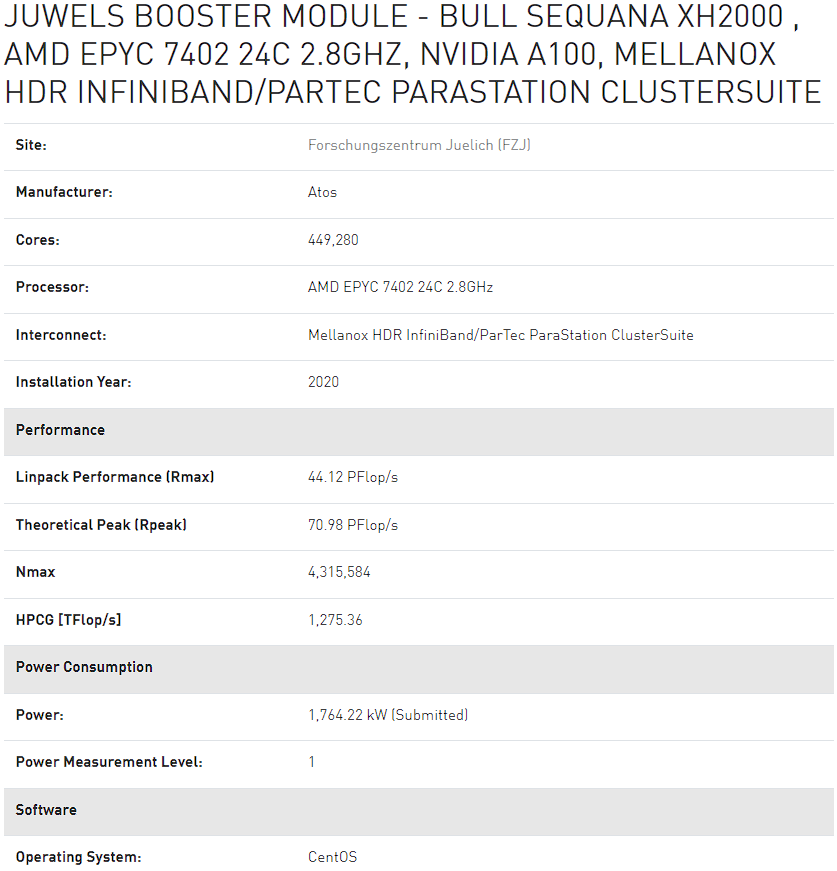
\includegraphics[width=\textwidth]{images/juwels_booster_top500.png}
    Aus: Top500, \url{https://www.top500.org/system/179894/} Zuletzt aufgerufen am: 20.06.2023
\end{bonus}

\begin{bonus}{Transistoren und Clock-Rate}
    Die Weiterentwicklung bei der Chipherstellung (Lithographie) führt zu feineren Strukturen auf einem Chip.
    
    Was passiert, wenn Leiterbahnen und Schaltelemente um einen Faktor $x$ schrumpfen ?
    \begin{itemize}
        \item Clock-Rate $f$ wächst um Faktor $x$ (Stromverbrauch, Abwärme $T \sim f^2$)
        \item Die Anzahl der Transistoren pro Fläche wächst mit $x^2$
        \item Die Rechenleistung des Chips wächst mit $x^4$ (aber der Zuwachs um $x^3$ beruht auf Architektur)
    \end{itemize}
\end{bonus}

\begin{defi}{Moore's Law}
    % TODO: https://de.wikipedia.org/wiki/Mooresches_Gesetz (Quelle)
    \emph{Moore's Law} besagt, dass sich die Komplexität integrierter Schaltkreise mit minimalen Komponentenkosten regelmäßig verdoppelt; je nach Quelle werden 12, 18 oder 24 Monate als Zeitraum genannt.
    
    Unter Komplexität verstand Gordon Moore, der das Gesetz 1965 formulierte, die Anzahl der Schaltkreiskomponenten auf einem integrierten Schaltkreis. Gelegentlich ist auch von einer Verdoppelung der Integrationsdichte die Rede, also der Anzahl an Transistoren pro Flächeneinheit.
\end{defi}

\begin{bonus}[Moore's Law]{Verlauf bis 2011}
    % TODO: https://simple.wikipedia.org/wiki/Moore%27s_law (Quelle)
    \centering
    
\includegraphics[width=0.75\textwidth]{images/moores_law.png}
\end{bonus}

\begin{bonus}{Leistungslücke Prozessor-Memory}
    Aufgrund von Moore's Law wächst die Leistungslücke (engl. \emph{Performance Gap}) um ca. 50\% pro Jahr, da bisher die CPU-Performance um ca. 60\% pro Jahr und die DRAM-Performance nur um ca. 7\% pro Jahr gewachsen ist.
    
    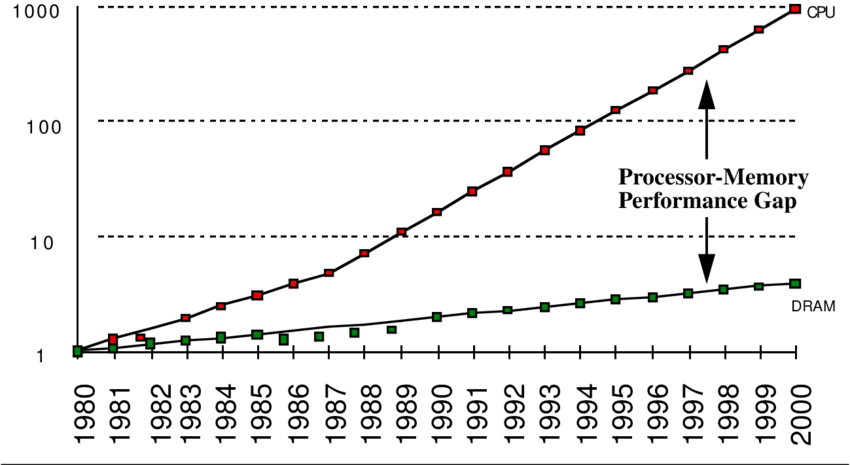
\includegraphics[width=\textwidth]{images/Processor-Memory-Performance-GapHen96.png}
    Katherine Yelick, \url{https://www.researchgate.net/figure/Processor-Memory-Performance-GapHen96_fig1_3214931}, zuletzt aufgerufen am: 20.06.2023
\end{bonus}

\section{Komplexität}\label{sec:komplexitaet}

\begin{defi}{Komplexität}
    Die \emph{Komplexität eines Algorithmus'} ist die Funktion $f(n)$, die den Aufwand für die benötigte Rechenzeit oder den benötigten Speicher in Abhängigkeit von der Problemgröße $n$ angibt.

    Die Komplexität ist abhängig von der Implementierung des Algorithmus'.

    Die \emph{Komplexität eines Problems} ist die minimale Komplexität aus einer Menge möglicher Algorithmen, die das Problem lösen.

    Die Komplexität ist \emph{unabhängig} von der Rechnerarchitektur.
\end{defi}

\begin{bonus}{Komplexitätsanalyse}
    Die \emph{Komplexitätsanalyse} untersucht z. B.:
    \begin{itemize}
        \item Wie viel Rechenzeit wird bei einer gegebenen Problemgröße $n$ benötigt?
        \item Wie ändert sich der Rechenzeitbedarf beim Anstieg von $n$?
        \item Ist der Rechenzeitbedarf noch realistisch und welcher Rechner kann das Problem in überschaubarer Zeit abarbeiten?
    \end{itemize}
\end{bonus}

\begin{defi}[Komplexität]{Problemgröße}
    Die \emph{Problemgröße} $n$ eines Programms bzw. Algorithmus' ist der Parameter, der den Aufwand für die benötigte Rechenzeit oder den benötigten Speicher bestimmt.
\end{defi}

\begin{defi}[Komplexität]{Rechenzeit}
    Die \emph{Rechenzeit} $T(n)$ eines Programms bzw. Algorithmus' ist die Anzahl der Rechenoperationen in Abhängigkeit von der Problemgröße $n$.

    Sie kann z. B. wie folgt berechnet werden:
    \[T(n) = a\cdot f(n) + t_b\]
    mit Rechenzeit $a$ für eine Rechen-, bzw. Gleitkomma-Operation und Rechenzeit $t_b$ für die Initialisierung und Beendigung des Algorithmus.
\end{defi}

\begin{defi}{Landau-Symbole}
    % TODO: https://de.wikipedia.org/wiki/Landau-Symbole (Quelle)
    \emph{Landau-Symbole} (auch \emph{O-Notation}) werden verwendet, um das asymptotische Verhalten von Funktionen und Folgen zu beschreiben.

    Die Komplexitätstheorie verwendet sie, um Probleme danach zu klassifizieren, wie \enquote{schwierig} oder aufwändig sie zu lösen sind.
    Zu \enquote{leichten} Problemen existiert ein Algorithmus, dessen Laufzeit sich durch ein Polynom beschränken lässt;
    als \enquote{schwer} gelten Probleme, für die man keinen Algorithmus gefunden hat, der weniger schnell als exponentiell wächst.

    % TODO: https://en.wikipedia.org/wiki/Big_O_notation (Quelle)
    Sei $f$ eine zu beschreibende reelle oder komplexe Funktion und $g$ eine reelle Vergleichsfunktion.

    $\mathcal{O}(g(n))$ bezeichnet eine Klasse von Funktionen, wobei
    \[ f(n) \in \mathcal{O}(g(n)) \]
    bedeutet, dass $f(n)$ höchstens so schnell wächst wie $g(n)$.
    Das widerum heißt, dass es zwei positive Konstanten $c$ und $n_0$ gibt, sodass
    \[ \forall n \geq n_0 : | f(n) | \leq c \cdot | g(n) | \]
\end{defi}

\begin{example}[Komplexitätsklassen]{Beschreibung}
    \begin{tabularx}{\linewidth}{llX}
        \toprule
        Klasse                  & Bezeichnung   & Beispiel                                                         \\
        \midrule
        $\mathcal{O}(1)$        & konstant      & Problem wird linear durchlaufen, unabhängig von Problemgröße     \\
        $\mathcal{O}(\log n)$   & logarithmisch & Binärsuche in einem sortierten Array                             \\
        $\mathcal{O}(n)$        & linear        & sequentielle Suche in einem unsortierten Array                   \\
        $\mathcal{O}(n \log n)$ & quasilinear   & \enquote{Divide-and-Conquer}-Algorithmen (Heap-Sort, Quick-Sort) \\
        $\mathcal{O}(n^2)$      & quadratisch   & einfache Sortieralgorithmen (Bubble-Sort, Selection-Sort)        \\
        $\mathcal{O}(n^c)$      & polynomiell   & Bestimmen der Determinante mithilfe von LU-Zerlegung             \\
        $\mathcal{O}(c^n)$      & exponentiell  & exaktes Lösen des Travelling-Salesman-Problems                   \\
        \bottomrule
    \end{tabularx}
\end{example}

\begin{example}[Komplexitätsklassen]{Visualisierung}
    \centering
    \begin{tikzpicture}[scale=1]
        \begin{axis}[
                width=15cm,
                unit vector ratio*=1 1,
                axis lines = middle,
                grid=major,
                ymin=0,
                ymax=50,
                xmin=0,
                xmax=50,
                xlabel = $n$,
                ylabel = $N$,
                xtick distance={5},
                ytick distance={5},
                disabledatascaling,
                cycle list name=color list,
                samples=250,
                solid,
                smooth,
                line width=1.0pt,
                no markers,
                legend cell align={left},
                reverse legend,
            ]

            \addplot +[domain=0:50]{0};         \addlegendentry{$\mathcal{O}(1)$};
            \addplot +[domain=0:50]{ln(x)};     \addlegendentry{$\mathcal{O}(\log(n))$};
                \addplot +[domain=0:50]{x};         \addlegendentry{$\mathcal{O}(n)$};
                \addplot +[domain=0:50]{x * ln(x)}; \addlegendentry{$\mathcal{O}(n \log(n))$};
            \addplot +[domain=0:50]{x^2};       \addlegendentry{$\mathcal{O}(n^2)$};
            \addplot +[domain=0:10]{2^x};        \addlegendentry{$\mathcal{O}(2^n)$};
        \end{axis}
    \end{tikzpicture}
\end{example}

\begin{example}[Komplexität]{Matrixmultiplikation}
    Problemgröße: $n$, ges.: $f(n)$ Anzahl der Rechen-Operationen in Abhängigkeit von der Matrix-Größe\\
    Notwendige Rechenzeit ist dann z.B.:
    \[T(n)=a\cdot f(n) + t_b\]
    mit $a$: Rechenzeit für eine Rechen- (Gleitkomma-) Operation,\\
    $b$: Rechenzeit für die Initialisierung und Beendigung des Algorithmus\\
    Formale Matrixmultiplikation:
    \[c_{i, j} = \sum\limits_{k=1}^{n}a_{i, k}\cdot b_{k, j}\]
    Bestimmung von $f(n)$: für jedes Element von $c$ sind $n$ Multiplikationen und $n-1$ Additionen durchzuführen.
    Also ergibt sich bei $n^2$ Elementen von $c$:
    \[f(n)=2\cdot n^3 - n^2\]

    TODO: Wording, Anschaulichkeit
\end{example}

\begin{bonus}{Master-Theorem}
    TODO
\end{bonus}

\begin{example}[Komplexität]{Strassen-Winograd}
    Effiziente Matrixmultiplikation:
    \begin{itemize}
        \item Matrizen werden in je vier Teilmatrizen der Größe $\frac{n}{2} \times \frac{n}{2}$ zerlegt:
              \begin{align*}
                  \begin{pmatrix}
                      A_{11} & A_{12} \\
                      A_{21} & A_{22}
                  \end{pmatrix}
                  \cdot
                  \begin{pmatrix}
                      B_{11} & B_{12} \\
                      B_{21} & B_{22}
                  \end{pmatrix}
                  =
                  \begin{pmatrix}
                      C_{11} & C_{12} \\
                      C_{21} & C_{22}
                  \end{pmatrix}
              \end{align*}
        \item Zusätzlich werden sieben neue Matrizen definiert:
              \begin{itemize}
                  \item $M_1 = (A_{12} - A_{22})\cdot(B_{21} + B_{22})$,
                  \item $M_2 = (A_{11} + A_{22})\cdot(B_{11} + B_{22})$,
                  \item $M_3 = (A_{11} - A_{21})\cdot(B_{11} + B_{12})$,
                  \item $M_4 = (A_{11} + A_{12})\cdot B_{22}$,
                  \item $M_5 = A_{11}\cdot(B_{21} - B_{22})$,
                  \item $M_6 = A_{22}\cdot(B_{21} - B_{11})$,
                  \item $M_7 = (A_{21} - A_{22})\cdot B_{11}$
              \end{itemize}
        \item Die vier Teilmatrizen der Ergebnismatrix ergeben sich damit wie folgt:
              \begin{itemize}
                  \item $C_{11} = M_1 + M_2 - M_4 + M_6$
                  \item $C_{12} = M_4 + M_5$
                  \item $C_{21} = M_6 + M_7$
                  \item $C_{22} = M_2 - M_3 + M_5 - M_7$
              \end{itemize}
    \end{itemize}
    Komplexität: $O(n^{\log_2 7})\approx O(n^{2.807})$
\end{example}
\section{Parallelverarbeitung}\label{sec:parallelverarbeitung}

\subsection{Parallele Bearbeitung einer Aufgabe}

\begin{defi}{Parallelverarbeitung}
    % TODO: https://de.wikipedia.org/wiki/Nebenl%C3%A4ufigkeit (Quelle)
    Die \emph{Parallelverarbeitung} (engl. \enquote{concurrency}), zielt darauf ab, mehrere Aufgaben, Berechnungen, Anweisungen oder Befehle gleichzeitig ausführen zu können.
    Es kann sich dabei um völlig unabhängige Anweisungen handeln, bis hin zur gemeinsamen Bearbeitung einer Aufgabe.
    
    Ziel ist eine \emph{Leistungssteigerung}.
    
    Voraussetzungen sind, dass
    \begin{itemize}
        \item eine Aufteilungsmöglichkeit existiert und erkannt wird,
        \item mehrere Bearbeiter zur Verfügung stehen und
        \item diese gleichzeitig und dabei möglichst unabhängig agieren können.
    \end{itemize}
\end{defi}

\begin{defi}{Domain Decomposition}
    \emph{Domain Decomposition} bzw. \emph{Gebietszerlegung} beschreibt die statische oder dynamische Aufteilung eines Datengebiets in Bereiche gleicher Prozessorarbeit.
    Alle Gebiete werden mit demselben Programmteil parallel verarbeitet.
    
    Domain Decomposition ist insbesondere geeignet für \emph{homogene Plattformen}, 
    wobei eine Kommunikation untereinander Voraussetzung ist.
    
    Im High-Performance-Computing (HPC) wird diese Art der Parallelisierung häufigsten verwendet.
\end{defi}

\begin{defi}[Domain Decomposition]{Statische Aufteilung}
    % TODO: https://de.wikipedia.org/wiki/Lastverteilung_(Informatik) (Quelle)
    \emph{Statische Aufteilung} der Domain Decomposition berücksichtigt den Zustand verschiedener Maschinen nicht.
    Sie soll z. B. die Kommunikation zwischen Prozessoren minimieren, oder bestimmte Hardware-Eigenschaften des Verbindungsnetzwerkes ausnutzen.
    
    Der Vorteil statischer Aufteilung ist, dass sie leicht zu implementieren und bei relativ regelmäßigen Aufgaben äußerst effizient ist.
\end{defi}

\begin{example}[Domain Decomposition]{Statische Aufteilung}
    TODO: Grafik
\end{example}

\begin{defi}[Domain Decomposition]{Dynamische Aufteilung}
    % TODO: https://de.wikipedia.org/wiki/Lastverteilung_(Informatik) (Quelle)
    \emph{Dynamische Aufteilung} der Domain Decomposition soll ein Gebiet in Bereiche gleicher Prozessorarbeit aufteilen.
    
    Im Gegensatz zur statischen Aufteilung wird bei der dynamische Variante die aktuelle Last jeder der Recheneinheiten im System berücksichtigt.
    Bei diesem Ansatz können Aufgaben dynamisch von einem überlasteten Knoten zu einem unterlasteten Knoten verschoben werden, um eine schnellere Verarbeitung zu erhalten.
    
    Obwohl diese Algorithmen viel komplizierter zu entwerfen sind, können sie hervorragende Ergebnisse liefern, insbesondere wenn die Ausführungszeit von einer Aufgabe zur anderen stark variiert.
    
\end{defi}

\begin{example}[Domain Decomposition]{Dynamische Aufteilung}
    TODO: Grafik
\end{example}

\begin{defi}{Functional Decomposition}
    \emph{Functional Decomposition} bzw. \emph{Funktionsaufteilung} beschreibt die Zerlegung eines Problems in unterschiedliche Programmteile, Unterprogramme oder Module, die dann auf Prozessoren verteilt und parallel bearbeitet werden.
    
    Dabei können die Programmteile auf jeweils unterschiedlichen, eventuell spezialisierten, Rechnerarchitekturen ausgeführt werden.
    
    Unterschiedliche Programmteile, Unterprogramme,
    Module werden auf Prozessoren verteilt und parallel bearbeitet.
    \begin{itemize}
        \item verschiedene Rechnerarchitekturen für unterschiedliche Programmteile einsetzbar
        \item aufwändiger zu Implementieren
    \end{itemize}
\end{defi}

\begin{jsc}[Functional Decomposition]{Modulare Supercomputing Architektur}
    % TODO: https://www.fz-juelich.de/de/ias/jsc/ueber-uns/struktur/forschungsgruppen/jsc-rg-proto/modulare-supercomputing-architektur (Quelle)
    Die \emph{Modular Supercomputing Architecture} (\emph{MSA}) ist ein Systemdesign zur Integration heterogener Ressourcen und zur Erfüllung der Anforderungen eines breiten Spektrums von Anwendungsbereichen, die von rechenintensiven, hochskalierenden Simulationscodes bis hin zu datenintensiven Workflows der künstlichen Intelligenz reichen.
    
    \vspace{1em}
    
    \centering
    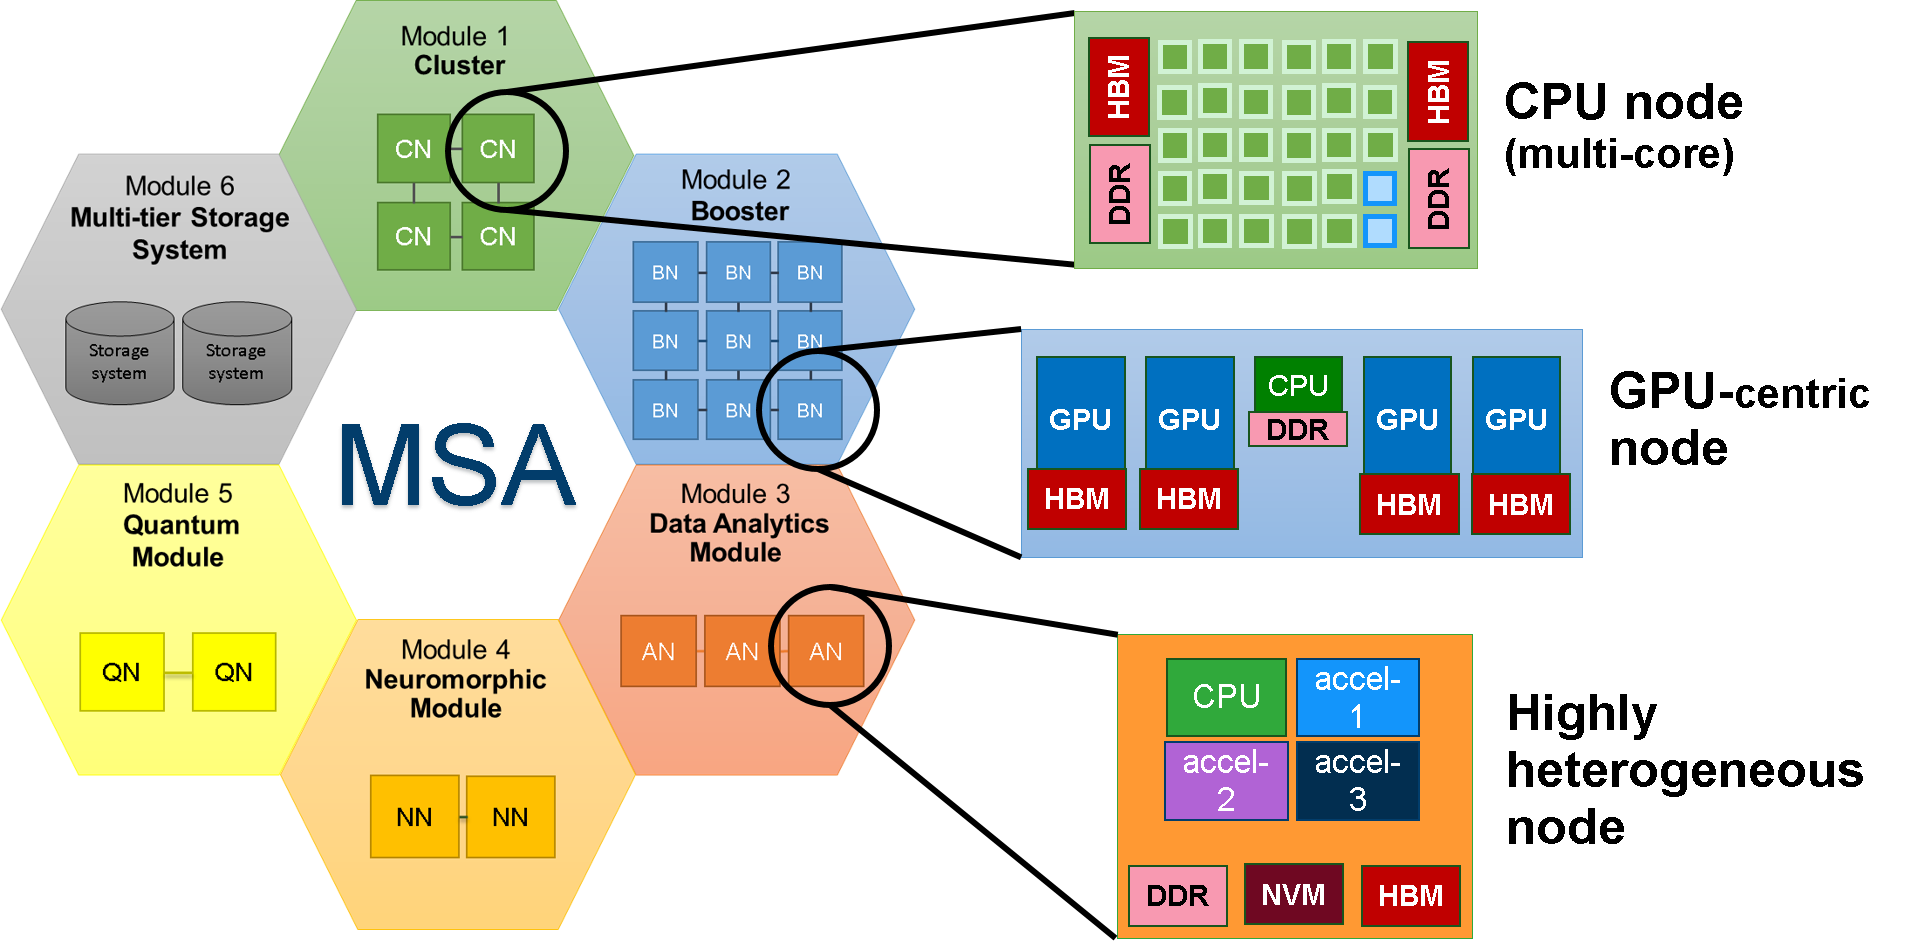
\includegraphics[width=0.9\linewidth]{images/modular_supercomputing_architecture.png}
\end{jsc}

\subsection{Speedup, Effizienz, Skalierbarkeit}

\begin{defi}{Speedup}
    % TODO: https://de.wikipedia.org/wiki/Speedup
    \emph{Speedup} beschreibt mathematisch den Zusammenhang zwischen der seriellen und der parallelen Ausführungszeit eines Programmteils.
    
    Der \emph{reale Speedup} $S$ einer parallelen Ausführung, der zur realen Messung herangezogen wird, kann wie folgt definiert werden:
    \[
        S = \frac{t_S}{t_p}
    \]
    Dabei sind $t_S$ und $t_p$ die serielle bzw. die parallele Ausführungszeit bei $p$ parallelen Bearbeitungseinheiten (Prozessoren).
\end{defi}

\begin{defi}{Amdahl's Law}
    % TODO: https://de.wikipedia.org/wiki/Speedup (Quelle)
    % TODO: https://de.wikipedia.org/wiki/Amdahlsches_Gesetz (Quelle)
    Das \emph{Amdahlsche Gesetz} (engl. \emph{Amdahl's Law}) ist ein Modell über die Beschleunigung von Programmen durch parallele Ausführung.
    Nach Amdahl wird der Geschwindigkeitszuwachs vor allem durch den sequentiellen Anteil des Problems beschränkt, da sich dessen Ausführungszeit durch Parallelisierung nicht verringern lässt.
    
    Der \emph{theoretische Speedup} $\eta_S$ nach Amdahl kann wie folgt definiert werden:
    \[
        \eta_S = \frac{t_S}{t_S \cdot f + t_S \cdot \frac{1-f}{p} } = \frac{t_S}{t_S \left((1 - f) + \frac{f}{n_P}\right)}
    \]
    Dabei sind $t_S$ und $t_p$ die serielle bzw. die parallele Ausführungszeit bei $p$ parallelen Bearbeitungseinheiten (Prozessoren);
    $f$ ist der Anteil der Laufzeit bzw. des Programms, der nicht parallel ablaufen kann und $n_P$ die Anzahl der Anzahl der Prozessoren, die zur Berechnung eingesetzt werden können.
    
    Es gelten weiterhin folgende Grenzwerte:
    \[
        \lim_{p \to \infty} \eta_S = \frac{1}{f} \quad \text{und} \quad \lim_{f \to 0 } \eta_S = n_P
    \]
\end{defi}

\begin{bonus}{Durchsatz}
    Der \emph{Speedup} ist ein Maß für die Bewertung der Verarbeitung eines einzelnen Programmteils, 
    während der \emph{Durchsatz} ein Maß für die Bewertung der Verarbeitung einer gesamten Arbeitslast ist.
    
    Beispiel: \emph{Speedup:} Zeit für einen einzelnen Passagier vs. 
    \emph{Durchsatz:} Anzahl der Passagiere pro Flug
    
    TODO: Definition
\end{bonus}

\begin{defi}{Effizienz}
    \emph{Effizienz} definiert das Verhältnis von Speedup und eingesetzter Prozessoranzahl.
    Sie drückt aus, welcher Anteil der Prozessorleistung nutzbar ist.
    
    Sie kann definiert werden als:
    \[
        E = \frac{S}{n_P} = \frac{t_S}{n_P\cdot t_P} \in (0, 1)
    \]
\end{defi}

\begin{example}[Speedup]{Skalarprodukt}
    Paralleler Algorithmus:
    \begin{enumerate}
        \item Aufteilen in $p$ Teilvektoren der Länge $\frac{n}{p}$
        \item jeder Prozessor berechnet das Skalarprodukt des Teilvektors $T_* (p) = \left(2 \cdot \frac{n}{p} - 1\right) \cdot t_\text{flop}$
        \item die Ergebnisse werden zu Prozessor 1 übertragen $T_t (p) = (p - 1) \cdot (t_\text{startup} + t_\text{word})$
        \item und Addition der Teilergebnisse (reduzieren) $T_+ (p) = (p - 1) \cdot t_\text{flop}$
    \end{enumerate}
    für $p=2^d$:
    \begin{align*}
        S(p) = \frac{T(\text{seq})}{T(p)} = \ldots =
        \frac{p}{\frac{p(\frac{2n}{p} + d-1)}{2n-1} + \frac{p\cdot d\cdot (t_\text{startup} + t_\text{word})}{(2n - 1)t_\text{flop}}}
    \end{align*}
    bei $n\gg p$:
    \begin{align*}
        \approx\frac{p}{
        \underbrace{1 + p\cdot \log_2 p}_{\text{Algorithmus}} \cdot
        \underbrace{\frac{1}{2n}}_{\text{Problemgröße}} \cdot
        \underbrace{\frac{t_\text{startup}}{t_\text{flop}}}_{\text{Hardware}}}
    \end{align*}
    
    TODO: Darstellung
\end{example}

\begin{example}[Effizienz]{Skalarprodukt}
    \[
        E(p) \approx \frac{1}{1 + n_P \cdot \log_2 n_P \cdot \frac{1}{2n} \cdot \frac{t_\text{startup}}{t_\text{flop}}}
    \]
    Die Effizienz
    \begin{itemize}
        \item \emph{steigt} mit wachsender Problemgröße $n$ (bei $n_P$ fest) und
        \item \emph{sinkt} bei größerer Prozessoranzahl $n_p$ (mit $n$ fest).
    \end{itemize}
    
    TODO: Darstellung\\
    TODO: Wie muss die Problemgröße $n$ wachsen bei festem $n_P$ und konstanter Effizienz?
\end{example}

\begin{defi}{Skalierbarkeit}
    Eine Rechnerarchitektur bzw. ein Programm ist \emph{skalierbar}, wenn die Effizienz der Programmbearbeitung bei wachsender Prozessorzahl gleich bleibt.
    Dies kann im Allgemeinen nur durch gleichzeitige Vergrößerung der Problemgröße erfolgen.
    
    Ein Programm bzw. ein Algorithmus ist \emph{perfekt skalierbar}, wenn $n \in \mathcal{O}(n_P)$ ist, also linear in $n_P$.
    
    TODO: Was soll das heißen?
\end{defi}

\begin{defi}{Paralleler Overhead}
    
    Der Speedup kann sich reduzieren durch zusätzlichen \emph{parallelen Overhead}.
    
    \[
        V(n_P) = n_P \cdot t_P - t_S
    \]
    
    Der \emph{durchschnittliche parallele Overhead} ist definiert als:
    \[
        \overline{V}(n_P) = \frac{V(n_P)}{n_P}
    \]
    
    Er wird verursacht durch:
    \begin{itemize}
        \item Kosten für das Starten eines Vorgangs (\enquote{startup}),
        \item Kosten für das Verteilen bzw. Verwalten gemeinsamer Daten, oder
        \item Kosten für Synchronisation.
    \end{itemize}
    
    Daher gilt abzuwägen zwischen:
    \begin{itemize}
        \item Verkleinern der Kommunikation durch größere Arbeitspakete (\emph{grobkörnige Granualität})
        \item Kleine Arbeitspaketen, damit viele Prozessoren arbeiten (\emph{feinkörnige Granualität})
    \end{itemize}
    
    TODO: Sinnvolle Definition finden
\end{defi}

% \begin{defi}{Pipelining}
%     \emph{Pipelining} beschreibt eine Implementierungstechnik, bei der komplexe Vorgänge in eine Sequenz von einfacheren Teilaufgaben zerlegt wird.

%     Die \emph{Stufen} der Pipeline (engl. \enquote{pipe stages}) werden hintereinander und verschachtelt ausgeführt.
%     Dabei sollen so viele Instruktionen wie möglich in einer Zeiteinheit ausgeführt werden, dadurch wird der Durchsatz erhöht.
%     Die Laufzeit einer einzelnen Pipeline bleibt jedoch unverändert.
% \end{defi}

\begin{defi}[Pipelining]{Speedup}
    Der bestmögliche \emph{Speedup} beim Pipelining entspricht der Anzahl der Pipeline-Stufen.
    Er wird reduziert durch unausgewogene Ausführungslängen.
    Die Geschwindigkeit der Pipeline ist also direkt beschränkt durch die langsamste Pipeline-Stufe.
    
    Eine effiziente Pipeline-Nutzung setzt voraus, dass eine möglichst hohe Anzahl von Aufträgen (Prozesse) verarbeitet wird.
    Bei nur einem Auftrag entartet die Pipeline zu einer reinen sequentiellen Verarbeitung.
    
    TODO: Formeln
\end{defi}

\begin{example}[Pipelining]{RISC vs. CISC}
    TODO: Grafik
\end{example}

\subsection{Aufgaben}

\begin{aufgabe}{Speedup}
    Ein sequentielles Programm lasse sich zu $80\%$ parallelisieren.
    Welcher Speedup kann mit 20 Prozessoren erzielt werden?
    \tcblower
    Der Speedup ist definiert durch:
    \begin{align*}
        \eta_S = \frac{t_S}{t_S \cdot f + t_S \cdot \frac{1-f}{p}}
    \end{align*}
    mit $t_S=1$, $f=1-0.8=0.2$, $p=20$ ist der Speedup eines Programmes dann:
    \begin{align*}
        \eta_S = \frac{1}{1 \cdot 0.2 + 1 \cdot \frac{0.8}{20}} = \frac{25}{6} \approx 4.1667
    \end{align*}
\end{aufgabe}

\begin{aufgabe}{Skalierbarkeit}
    Wann ist eine Rechnerarchitektur bzw. ein Programm skalierbar?
    \tcblower
    Wenn die Effizienz der Programmbearbeitung bei wachsender Prozessorzahl gleich bleibt.
\end{aufgabe}

\begin{aufgabe}{Pipelining}
    Wie berechnet sich der Speedup $\eta_S$ bei Pipeline-Nutzung mit n Aufträgen und k Stufen?
    \tcblower
    Der Speedup berechnet sich durch:
    \begin{align*}
        \eta_S = \frac{n\cdot k}{n+k-1}
    \end{align*}
\end{aufgabe}

\section{Einzelprozessorsysteme}\label{sec:einzelprozessorsysteme}

\begin{defi}{Überlappte Verarbeitung}
    Ein erstes Ziel der Parallelität war die \emph{überlappte Verarbeitung} von langsamen und schnellen Hardware-Komponenten.
\end{defi}

\begin{example}[Überlappte Verarbeitung]{Direct Memory Access}
    % TODO: https://de.wikipedia.org/wiki/Direct_Memory_Access (Quelle)
    Unter \emph{Direct Memory Access} versteht man, wenn Hardware-Komponenten selbstständig ohne Beteiligung der CPU Daten übertragen können.
    Diese Technik erlaubt anderen Komponenten ohne Umweg über die CPU direkt mit dem Arbeitsspeicher zu kommunizieren.
    
    Der Vorteil des DMA ist die schnellere Datenübertragung bei gleichzeitiger Entlastung des Prozessors.
    
    Anders als der Name vermuten lässt, ist die wesentliche Eigenschaft von Direct Memory Access nicht der Speicherzugriff, sondern dass der Datentransfer von einer anderen Komponente und nicht von der CPU selbst initiiert wird. Dabei braucht es zu keinen Speicherzugriffen zu kommen, es sind auch direkte Kommunikationen zwischen Peripheriegeräten möglich
    
    TODO: Grafik
\end{example}

\begin{defi}{Überlappter I/O}
    TODO: Sinnvolle Definition und Voraussetzungen
    
    TODO: Grafik
    
    Während des langsamen I/O kann nun gleichzeitig die \enquote{wertvolle} Ressource CPU genutzt werden.
\end{defi}

\subsection{Cache}\label{subsec:cache}

\begin{defi}{Cache}
    % TODO: https://de.wikipedia.org/wiki/Cache (Quelle)
    \emph{Cache} bezeichnet einen schnellen Pufferspeicher, der (wiederholte) Zugriffe auf ein langsames Hintergrundmedium oder aufwendige Neuberechnungen zu vermeiden hilft.
    
    Daten, die bereits einmal geladen oder generiert wurden, verbleiben im Cache, so dass sie bei späterem Bedarf schneller aus diesem abgerufen werden können.
    
    Auch können Daten, die vermutlich bald benötigt werden, vorab vom Hintergrundmedium abgerufen und vorerst im Cache bereitgestellt werden (\emph{read-ahead}).
    
    Da es technisch aufwändig und damit meist wirtschaftlich nicht sinnvoll ist, einen Cache zu bauen, der sowohl groß als auch schnell ist, kann man mehrere Caches verwenden -- z. B. einen kleinen schnellen und einen deutlich größeren, jedoch etwas langsameren Cache (der aber immer noch viel schneller ist als der zu cachende Hintergrundspeicher).
    
    Damit kann man die konkurrierenden Ziele von geringer Zugriffszeit und großem Cacheumfang gemeinsam realisieren.
    Das ist wichtig für die \emph{Hit Rate}.
\end{defi}

\begin{defi}{Cachehierarchie}
    Existieren mehrere Caches, so bilden diese eine \emph{Cachehierarchie}, die Teil der Speicherhierarchie ist.
    
    Die einzelnen Caches werden nach ihrer Hierarchieebene (engl. \emph{level}) durchnummeriert, also Level-1 bis Level-n oder kurz L1, L2 usw.
    Je niedriger die Nummer, desto näher liegt der Cache an der (schnell) verarbeitenden Komponente;
    die niedrigste Nummer bezeichnet daher den Cache mit der schnellsten Zugriffszeit, dieser wird als erstes durchsucht.
    
    Enthält der L1-Cache die benötigten Daten nicht, wird der (meist etwas langsamere, aber größere) L2-Cache durchsucht usw.
    Das geschieht solange, bis die Daten entweder in einer Cacheebene gefunden (\emph{Cache Hit}) oder alle Caches ohne Erfolg durchsucht wurden (\emph{Cache Miss}).
    In letzterem Fall muss auf den langsamen Hintergrundspeicher zugegriffen werden.
\end{defi}

\begin{example}[Cachehierarchie]{IBM Power 4}
    TODO
\end{example}

\begin{example}[Cachehierarchie]{Intel Itanium}
    TODO
\end{example}

\begin{example}[Cachehierarchie]{Harvard-Architektur}
    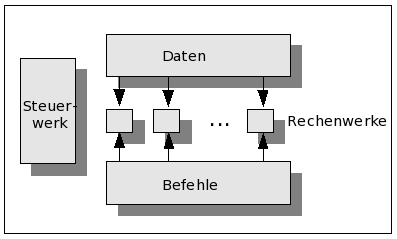
\includegraphics[width=\textwidth]{images/harvard_architektur.png}
    Von Matthias Kleine (April 2005) - \url{Matthias Kleine, CC BY-SA 3.0, https://de.wikipedia.org/w/index.php?curid=624441}, zuletz aufgerufen am: 19.06.2023
    % TODO: https://en.wikipedia.org/wiki/Cache_hierarchy (Quelle, Grafiken)
\end{example}

\begin{defi}[Cache]{Zugriffszeit}
    Durch die Aufteilung des L1-Cache in Daten- und Instruktions-Cache (Harvard-Architektur) können bei Pipeline-basierten Rechnern gleichzeitig neue Instruktionen zum Füllen der Pipeline geholt werden und bei der Bearbeitung der Operanden die Daten ausgelesen werden.
    
    Die \emph{Zugriffszeit} $t_Z$ eines Caches kann wie folgt definiert werden:
    \[
        t_Z = t_{C} + (1 - h) \cdot t_{M}
    \]
    Dabei ist $t_C$ die Zugriffszeit des Prozessors für Werte aus dem Cache, $t_M$ die für Daten aus dem Memory und $h$ die Hit-Rate.
    
    Wenn die Hit-Rate groß sein soll, sind sowohl ein Programm mit hoher räumlicher und zeitlicher Lokalität, sowie ein großer Cache (meist L1, L2 und L3) erforderlich.
\end{defi}

\begin{defi}{Cache Hits und Misses}
    % TODO: https://de.wikipedia.org/wiki/Cache#Organisation (Quelle)
    Den Vorgang, dass die Daten einer Anfrage an einen Cache in selbigem vorrätig sind, bezeichnet man als \emph{Cache Hit}, den umgekehrten Fall als \emph{Cache Miss}.
    
    Man unterscheidet zwischen folgenden Cache Misses:
    \begin{itemize}
        \item \emph{Cold Start Miss}; tritt auf beim ersten Zugriff auf einen Block nach dem Start des Programms oder dem Task-Wechsel.
        \item \emph{Capacity Miss}; tritt auf, wenn der Cache nicht alle Blocks speichern kann, die bei der Ausführung durch die CPU benötigt werden (nur bei Fully Associative Cache).
        \item \emph{Conflict Miss}; tritt auf, wenn ein Block ersetzt werden muss, der anschließend wieder benötigt wird (bei N-way Set Associative Cache).
        \item \emph{Coherence Miss}; bei Mehrprozessorsystemen.
    \end{itemize}
\end{defi}

\begin{defi}{Hit und Miss Rate}
    % TODO: https://de.wikipedia.org/wiki/Cache#Organisation (Quelle)
    Um quantitative Maßzahlen für die Bewertung der Effizienz eines Caches zu erhalten, definiert man zwei Größen.
    
    Die Anzahl der Anfragen, bei denen ein Cache Hit auftrat, geteilt durch die Anzahl der insgesamt an diesen Cache gestellten Anfragen bezeichnet man als \emph{Hit Rate}.
    Wie man aus der Definition leicht sehen kann, liegt diese Größe zwischen Null und Eins. Eine Hit Rate von z. B. 70 \% bedeutet, dass bei 70 \% aller Anfragen an den Cache dieser die Daten sofort liefern konnte und bei 30 \% aller Anfragen passen musste.
    
    Analog zur Hit Rate ist die \emph{Miss Rate} als die Anzahl der Anfragen definiert, bei denen die Daten nicht im Cache vorhanden waren geteilt durch die Anzahl der gesamten Anfragen.
    Offensichtlich gilt:
    \[
        \text{Miss Rate} = 1 - \text{Hit Rate}
    \]
\end{defi}

\begin{defi}{Cache-Assoziativität}
    Die Cache-Lines (Blöcke) eines Caches können in so genannte \emph{Sätze} zusammengefasst werden.
    Für eine bestimmte Adresse ist dann immer nur einer der Sätze zuständig.
    Innerhalb eines Satzes bedienen alle Cache-Lines also nur einen Teil aller vorhandenen Adressen.
    
    Im Folgenden stehe die Variable $m$ für die Gesamtanzahl der Cache-Liness und $n$ für die Anzahl der Cache-Lines pro Satz, die so genannte \emph{Assoziativität}.
    Dann besteht der Cache also aus $\frac{m}{n}$ Sätzen.
\end{defi}

\begin{defi}[Cache-Assoziativität]{Direct Mapped Cache}
    % TODO: https://en.wikipedia.org/wiki/Cache_placement_policies#Direct-mapped_cache (Quelle)
    Bei einem \emph{Direct Mapped Cache} wird jeder Block repräsentiert einen durch eigenen Satz, es gibt also so viele Sätze wie Cache-Lines.
    Somit ist für eine gegebene Adresse exakt ein Cacheblock zuständig.
    
    Platzieren eines Speicherblocks im Cache:
    \begin{itemize}
        \item Bestimmen der Zeilenadresse im Cache, basierend auf Adresse im Hauptspeicher
        \item Speicherblock wird entsprechend im Cache gespeichert, als Tag wird die Hauptspeicheradresse verwendet
        \item vorher gespeicherte Daten werden überschrieben
    \end{itemize}
    
    Suchen im Cache:
    \begin{itemize}
        \item Bestimmen der Zeilenadresse im Cache, basierend auf Adresse im Hauptspeicher
        \item Tags (Hauptspeicheradressen) werden verglichen
        \item bei gleichen Tags \emph{Cache-Hit}, sonst \emph{Cache-Miss}
        \item bei einem Cache-Miss muss der Speicherblock in den Cache geladen werden
    \end{itemize}
    
    Vorteile des Direct Mapped Cache sind, dass nicht alle Adressen im Cache durchsucht werden müssen und das Vorgehen sehr simpel ist.
    
    Im Gegenzug ist die Effizienz des Caches eingeschränkt, da möglicherweise freie Cacheblöcke vorhanden sind, die nicht genutzt werden.
    
    \centering
    % TODO: https://diveintosystems.org/book/C11-MemHierarchy/caching.html (Quelle)
    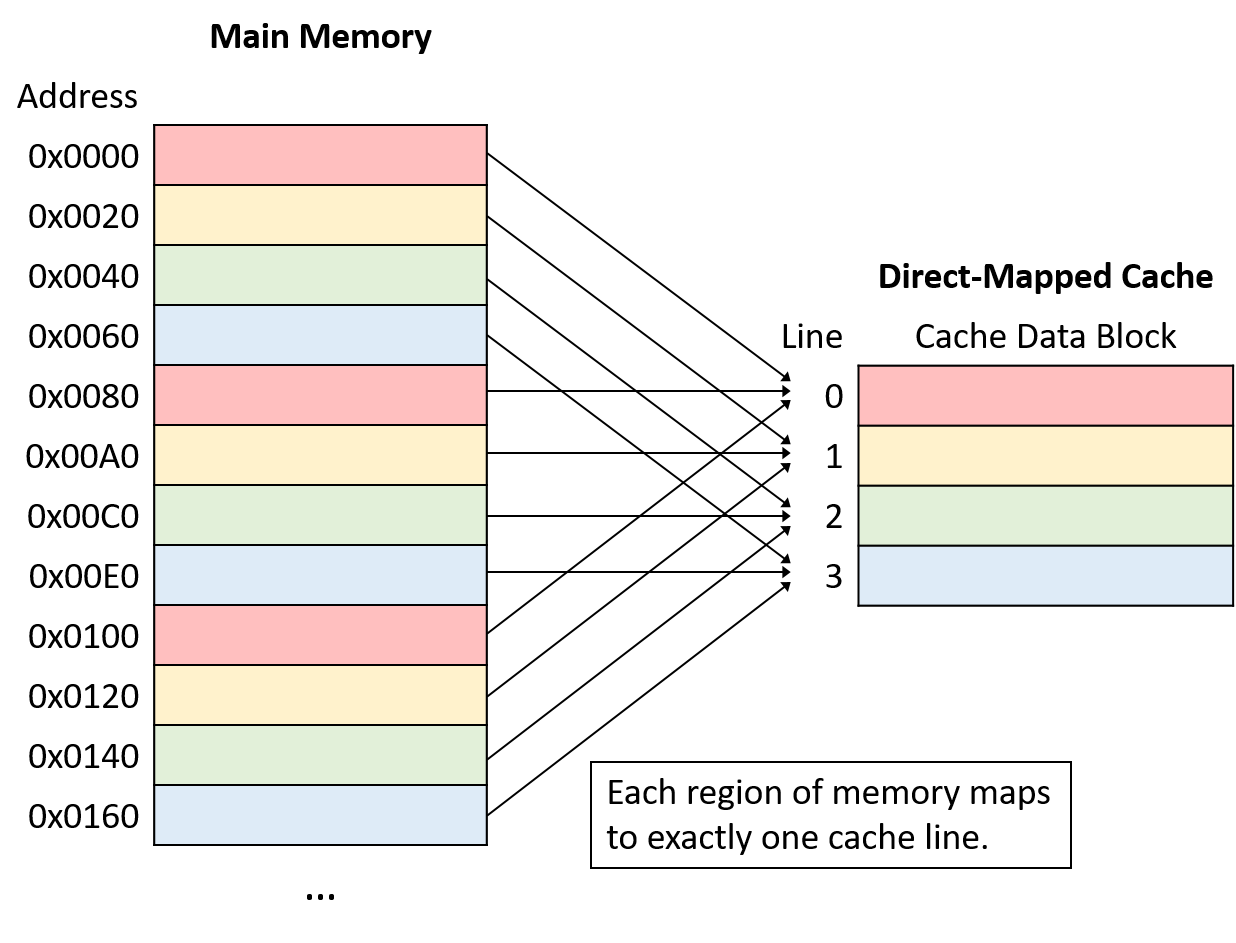
\includegraphics[width=.6\linewidth]{images/direct_mapped_cache.png}
    % 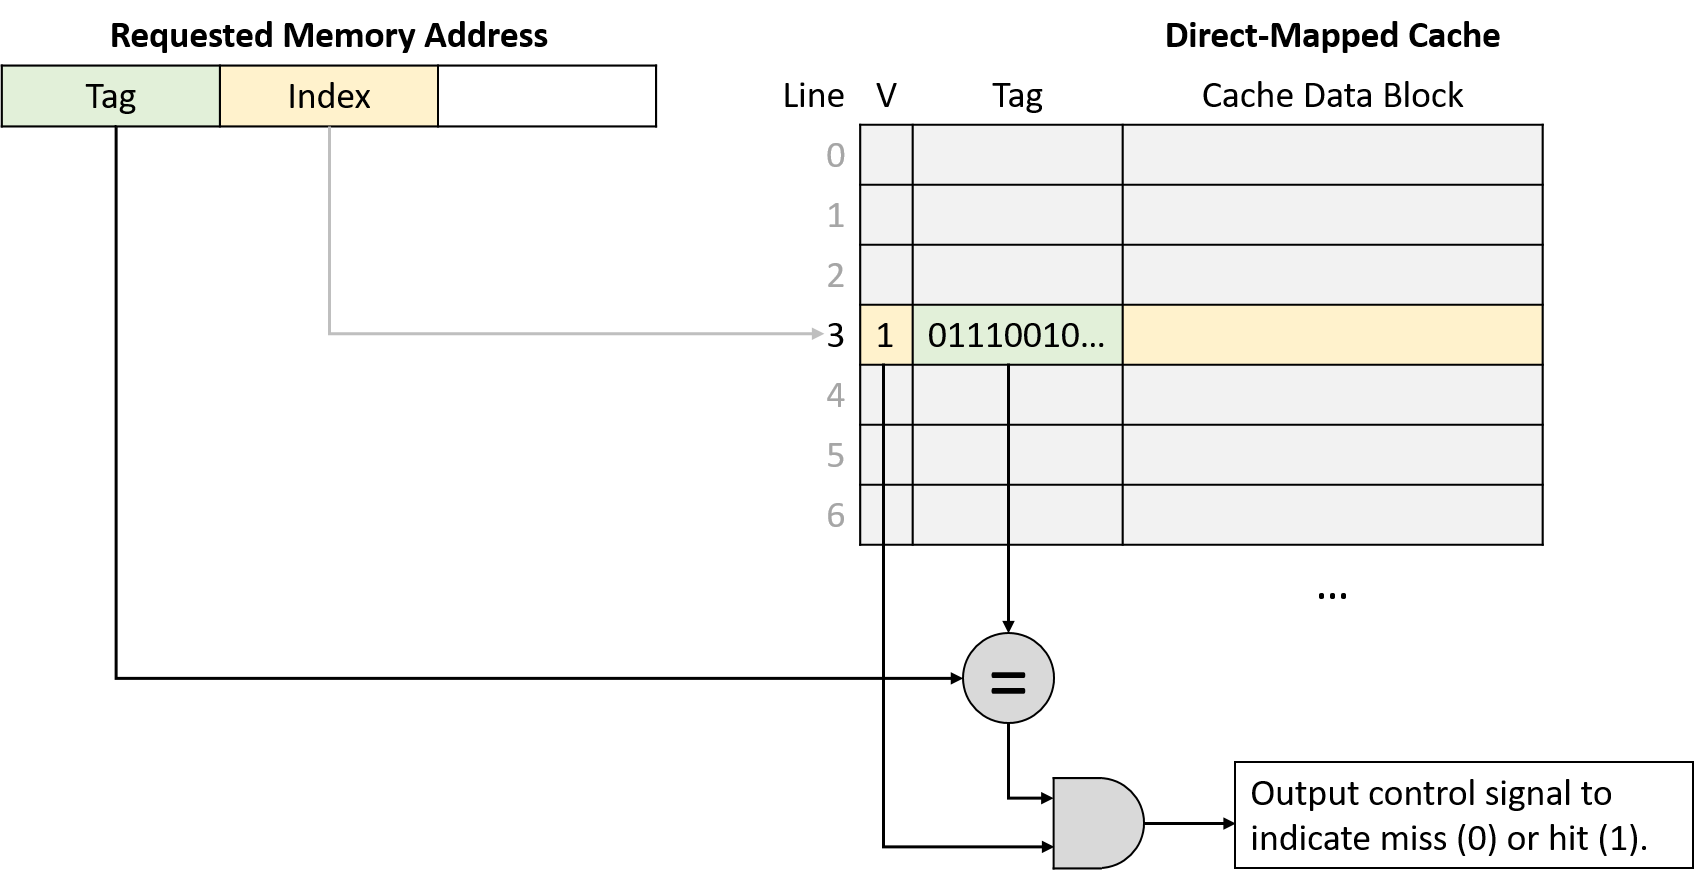
\includegraphics[width=.9\linewidth]{images/direct_mapped_cache_request.png}
\end{defi}

\begin{defi}[Cache-Assoziativität]{Fully Associative Cache}
    % TODO: https://de.wikipedia.org/wiki/Cache#Organisation (Quelle)
    Ein \emph{Fully Associative Cache} hat nur einen Satz, der alle Blöcke beinhaltet.
    Somit kann jede Adresse in jedem Cacheblock gecached werden.
    
    Bei einer Anfrage an den Cache ist es daher notwendig, alle Cache-Tags zu überprüfen.
    Da Caches möglichst schnell sein müssen, wird das parallel ausgeführt, was den notwendigen Hardwareaufwand an Tag-Vergleichern vergrößert.
    
    Der Vorteil ist aber, dass der Cache stets Daten aufnehmen kann, solange noch ein beliebiger Cacheblock frei ist.
\end{defi}

\begin{defi}[Cache-Assoziativität]{N-way Set Associative Cache}
    % TODO: https://de.wikipedia.org/wiki/Cache#Organisation (Quelle)
    Ein \emph{N-way Set Associative Cache} reduziert Konflikte beim Zwischenlagern im Cache durch $N$ \emph{Cache-Sets}.
    
    Beim \emph{2-way Set Associative Cache} werden bei der Anforderung einer Hauptspeicheradresse in den beiden Cache-Sets parallel an der entsprechenden Stelle der Tag verglichen.
    Stimmt ein Tag überein, kann direkt aus dem Cache gelesen werden (\emph{Cache-Hit}).
    Sind beide Tags verschieden, muss in einem Cache-Set eine Zeile neu aus dem Hauptspeicher geladen werden (\emph{Cache-Miss}).
    
    Diese Cacheform stellt einen Kompromiss aus Hardwareaufwand und Effizienz des Caches dar:
    Gegenüber einem DM-Cache gewinnt man Effizienz, gegenüber einem FA-Cache spart man Hardware.
    
    % TODO: https://diveintosystems.org/book/C11-MemHierarchy/caching.html (Quelle)
    \centering
    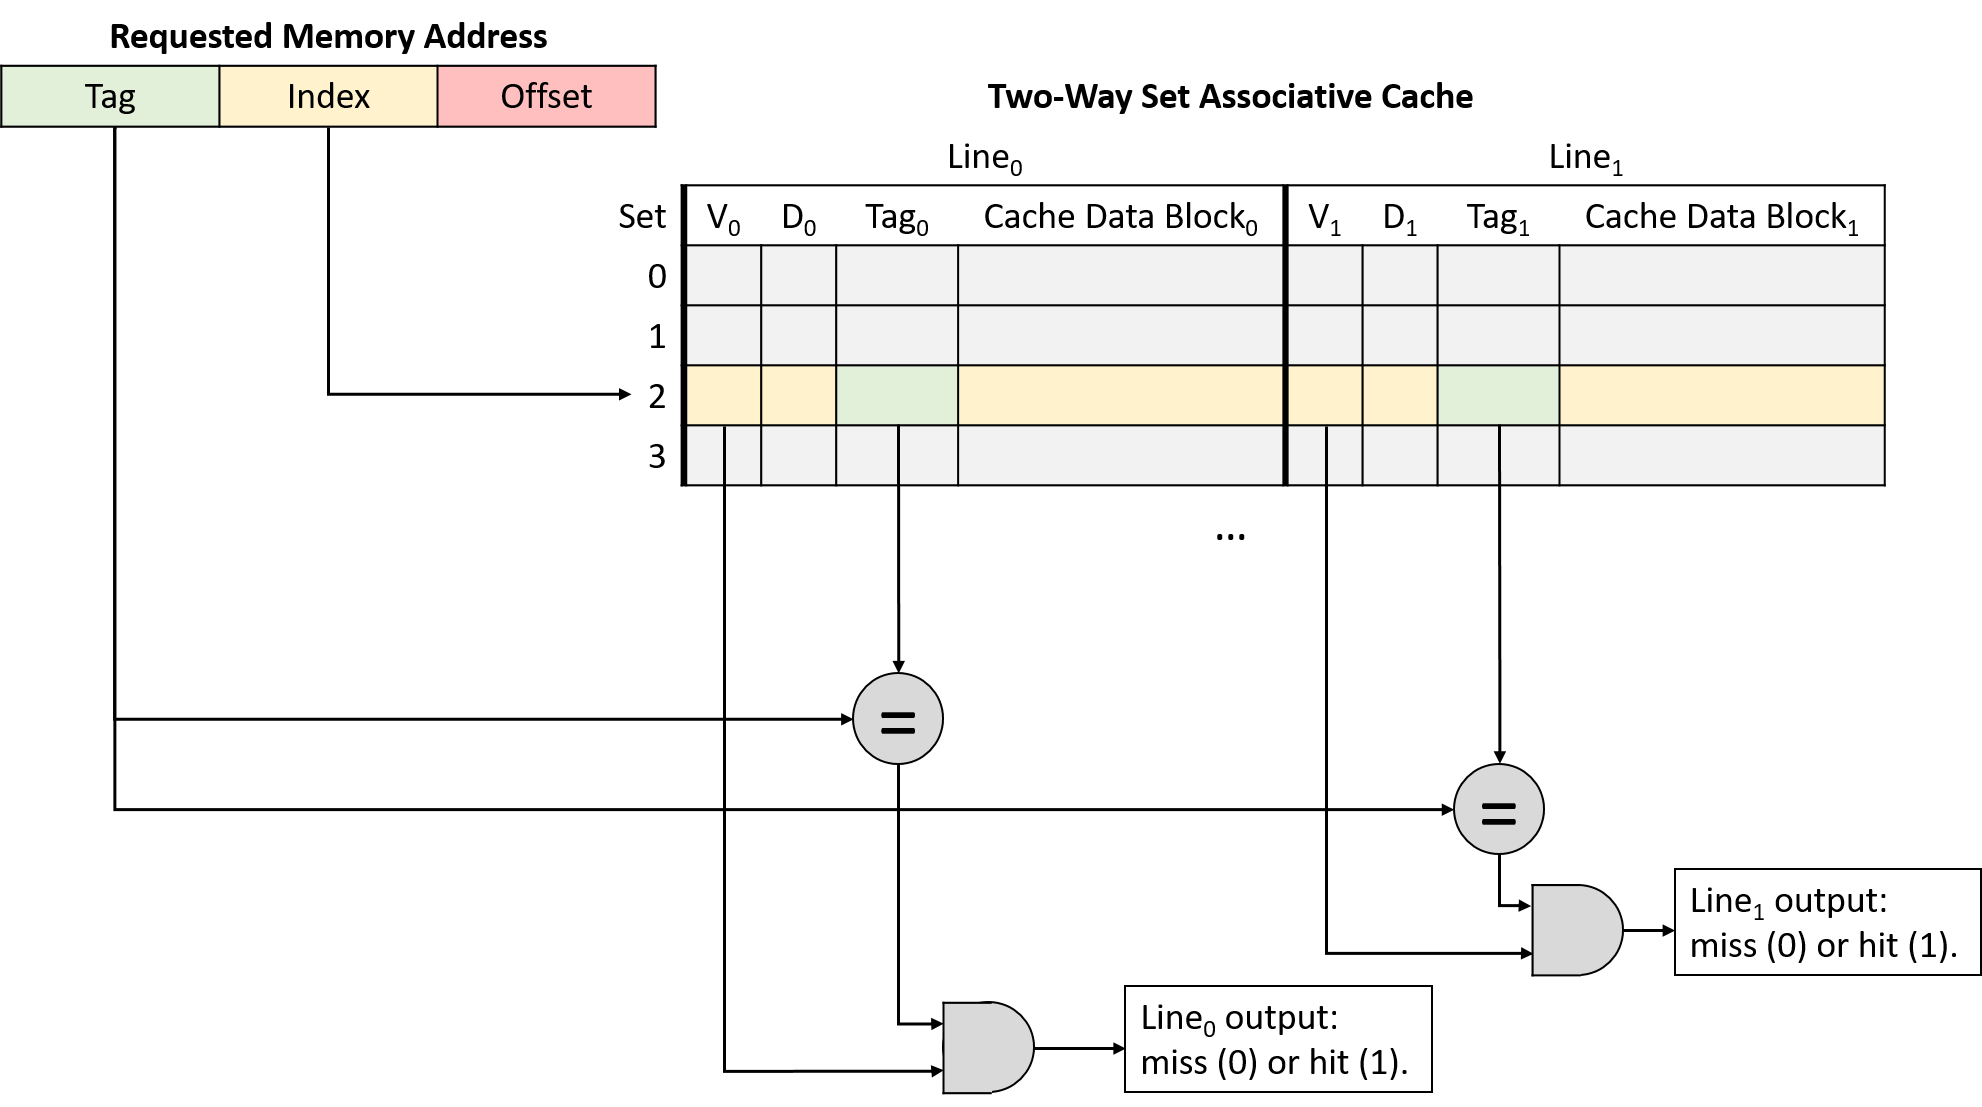
\includegraphics[width=.9\linewidth]{images/2-way_set_associative_cache_request.png}
\end{defi}

\begin{defi}{Ersetzungsstrategie}
    % TODO: https://de.wikipedia.org/wiki/Cache#Organisation (Quelle)
    Bei der Verwaltung des Caches ist es sinnvoll, immer nur die Blöcke im Cache zu halten, auf die auch häufig zugegriffen wird.
    Zu diesem Zweck gibt es verschiedene \emph{Ersetzungsstrategien}.
\end{defi}

\begin{defi}[Ersetzungsstrategie]{LRU}
    Eine häufig verwendete Ersetzungsstrategie ist die \emph{LRU} (engl. Least Recently Used), 
    bei welcher immer der Block ausgetauscht wird, auf den am längsten nicht mehr zugegriffen wurde.
    
    Moderne Prozessoren (z. B. der AMD Athlon) implementieren meist eine Pseudo-LRU-Ersetzungsstrategie, die fast wie echtes LRU arbeitet, aber leichter in Hardware zu implementieren ist.
\end{defi}

\begin{defi}[Ersetzungsstrategie]{FIFO}
    Ähnlich funktioniert die \emph{FIFO-Strategie} (engl. First In First Out), 
    bei der schlicht der jeweils älteste Eintrag verdrängt wird.
\end{defi}

\begin{defi}[Ersetzungsstrategie]{Random}
    Ebenfalls üblich ist, dass ein zufälliger Eintrag verdrängt wird (\emph{Random-Strategie}).
    
    Meistens wird diese \emph{Ersetzungsstrategie} genommen, 
    da diese am einfachsten zu implementieren ist, 
    kein Overhead produziert und gleiche Leistung bringt.
\end{defi}

\begin{defi}{Schreibstrategie}
    Bei einem Schreibzugriff muss generell unterschieden werden, ob ein Block bereits im Cache, oder noch ungeladen im Hauptspeicher ist.
    Es muss also eine \emph{Schreibstrategie} gewählt werden.
    
    Bei einem Schreibzugriff auf einen Block, der im Cache vorhanden ist, gibt es prinzipiell zwei Möglichkeiten:
    \begin{itemize}
        \item Durchgängiges Schreiben (Write-Through)
        \item Zurückkopieren (Write-Back)
    \end{itemize}
    
    Analog zu Obigem gibt es bei einem Schreibzugriff auf einen Block, der nicht im Cache vorhanden ist, prinzipiell ebenso zwei Möglichkeiten:
    \begin{itemize}
        \item Write-Allocate
        \item Non-Write-Allocate
    \end{itemize}
    
    Einige Befehlssätze enthalten Befehle, die es dem Programmierer ermöglichen, explizit anzugeben, ob zu schreibende Daten am Cache vorbeizuschreiben sind.
    
    Normalerweise wird entweder die Kombination Write-Back mit Write-Allocate oder Write-Through mit Non-Write-Allocate verwendet.
    Die erste Kombination hat den Vorteil, dass aufeinander folgende Schreibzugriffe auf denselben Block (Lokalitätsprinzip) komplett im Cache abgewickelt werden (bis auf den ersten Miss).
    Dies gibt im zweiten Fall keinen Vorteil, da sowieso jeder Schreibzugriff zum Hauptspeicher muss, weshalb die Kombination Write-Through mit Write-Allocate eher unüblich ist.
\end{defi}

\begin{defi}[Schreibstrategie]{Write-Through}
    % TODO: https://de.wikipedia.org/wiki/Cache#Organisation (Quelle)
    Bei \emph{Write-Through} wird der zu schreibende Block sofort in der nächsthöheren Speicherebene abgelegt.
    Damit ist die Konsistenz gesichert.
    
    Damit der Prozessor nicht jedes Mal warten muss, bis der Block in der nächsthöheren Speicherebene (die ja langsamer als der Cache ist) abgelegt ist, benutzt man einen Pufferspeicher (write buffer).
    Wenn dieser voll läuft, muss der Prozessor jedoch anhalten und warten.
\end{defi}

\begin{defi}[Schreibstrategie]{Write-Back}
    % TODO: https://de.wikipedia.org/wiki/Cache#Organisation (Quelle)
    Bei \emph{Write-Back} wird der zu schreibende Block nicht sofort in der nächsthöheren Speicherebene abgelegt, sondern zunächst im Cache.
    
    Dabei entsteht eine Inkonsistenz zwischen Cache und zu cachendem Speicher.
    Letzterer enthält somit veraltete Information.
    Erst wenn das Wort aus dem Cache verdrängt wird, wird es auch in die nächsthöhere Speicherebene geschrieben.
    Dazu bekommt jeder Cacheblock ein sogenanntes Dirty Bit, das anzeigt, ob der Block beim Ersetzen zurückkopiert werden muss.
    
    Das führt bei Speicherzugriff durch andere Prozessoren oder DMA-Geräte zu Problemen, weil diese veraltete Informationen lesen würden.
    Abhilfe schaffen hier Cache-Kohärenz-Protokolle wie z. B. MESI für UMA-Systeme.
    
    Ein Vorteil ist, dass mehrfaches Ändern eines Wertes nur im Cache durchgeführt wird.
    Allerdings kann ein Read-Miss zu einem Schreiben in den Hauptspeicher führen.
\end{defi}

\begin{bonus}[Schreibstrategie]{Write-Allocate}
    % TODO: https://de.wikipedia.org/wiki/Cache#Organisation (Quelle)
    Wie bei einem normalen Cache Miss wird bei \emph{Write-Allocate} der Block aus der nächsthöheren Speicherebene geholt.
    Die entsprechenden Bytes, die durch den Schreibzugriff geändert wurden, werden danach im gerade frisch eingetroffenen Block überschrieben.
\end{bonus}

\begin{bonus}[Schreibstrategie]{Non-Write-Allocate}
    % TODO: https://de.wikipedia.org/wiki/Cache#Organisation (Quelle)
    Bei \emph{Non-Write-Allocate} wird am Cache vorbei in die nächsthöhere Speicherebene geschrieben, ohne dass der dazugehörige Block in den Cache geladen wird.
    
    Das kann für manche Anwendungen Vorteile bringen, bei denen viele geschriebene Daten nie wieder gelesen werden.
    Durch die Verwendung von Non-Write-Allocate verhindert man das Verdrängen von anderen, möglicherweise wichtigen Blöcken und reduziert somit die Miss Rate.
\end{bonus}

\begin{defi}[Reduzierung der Cache Miss Rate]{Programmierstrategien}
    Verbessern der Speicherlokalität durch
    \begin{itemize}[\ldots]
        \item Datenstrukturierung
        \item Ändern der Indexierung
        \item Schleifenfusion
        \item Bildung von Teilblöcken
    \end{itemize}
\end{defi}

\begin{example}[Reduzierung der Cache Miss Rate]{Programmierung}
    TODO: Beispiel Umsortierung der Schleifen um Zeilen und Spalten einer Matrix andersrum zu durchlaufen.
\end{example}

\begin{defi}{Translation-Lookaside-Buffer}
    % TODO: https://de.wikipedia.org/wiki/Translation_Lookaside_Buffer (Quelle)
    Der Begriff \emph{Übersetzungspuffer} bzw. \emph{Translation Lookaside Buffer} (\emph{TLB}) bezeichnet eine funktionale Einheit der Speicherverwaltung.
    
    Wenn virtueller Speicher verwendet wird, muss zu den virtuellen Adressen die jeweils zugehörige physische Adresse ermittelt werden.
    Da diese Arbeitsschritte verhältnismäßig zeitintensiv sind, werden die zuletzt ermittelten $n$ Werte für die Adresse der physischen Speicherseite im TLB zwischengespeichert, wodurch erneute Zugriffe auf Adressen in dieser Seite nicht aufwändig neu ermittelt werden müssen, sondern aus dieser Liste entnommen werden können.
    
    Der TLB kann eine begrenzte Menge dieser Referenzen halten (üblicherweise nicht mehr als 1024 Einträge) und kann dadurch die Ausführung von Speicherzugriffen deutlich beschleunigen.
    
    Bei Rechnern mit virtuellen Adressen wird bei einem Task-Wechsel zu Beginn der Cache invalidiert.
    Daher kommt es für die neue Task zu Cold Start Misses!
    
    TODO: Grafik
\end{defi}

\subsection{Entwicklungslinien der Prozessoren}\label{subsec:entwicklungslinien-der-prozessoren}

\begin{defi}[Befehlssatzarchitektur]{CISC}
    % TODO: https://de.wikipedia.org/wiki/Complex_Instruction_Set_Computer (Quelle)
    Anfänglich wurden die Befehlssätze der Prozessoren immer umfangreicher, um auch komplexere Rechenschritte \enquote{auf einmal} mit nur einem Maschinenbefehl ausführen zu können, 
    um dadurch schneller und leistungsfähiger zu werden.
    Zugleich wurde dadurch jedoch auch der Prozessor komplex und schwierig weiterzuentwickeln, sowie auch schwieriger zu programmieren.
    
    Viele Hersteller setzten zunächst auf die Mikroprogrammierung der Rechenwerke, um Problemfälle leichter korrigieren zu können -- dennoch nahm die Komplexität immer weiter zu.
    
    Die Bezeichnung \emph{Complex Instruction Set Computer} (\emph{CISC}) wurde in den 1970er Jahren von IBM als Retronym gewählt, um klassische Befehlssätze von einer neuartigen Form abzugrenzen, dem Reduced Instruction Set Computer (RISC).
    
    TODO: Grafik
\end{defi}

\begin{defi}[Befehlssatzarchitektur]{RISC}
    % TODO: https://de.wikipedia.org/wiki/Reduced_Instruction_Set_Computer (Quelle)
    \emph{Reduced Instruction Set Computer} (\emph{RISC}) ist eine Designphilosophie für Computerprozessoren.
    Das Designziel war der Verzicht auf einen komplexen, 
    für die Assemblerprogrammierung komfortablen Befehlssatz hin zu einfach zu dekodierenden und schnell auszuführenden Befehlen (\enquote{eigentliche Befehlsausführung} meist nur 1 Takt).
    Dies ermöglichte zudem höhere Taktfrequenzen.
    
    Der Compiler erzeugt direkt Mikrobefehle.
    Es muss zwar mehr Code erzeugt werden, aber die Hardware wird einfacher und damit auch schneller.
    
    TODO: Grafik
\end{defi}

\subsection{Aufgaben}

\begin{aufgabe}[Caches]{Ersetzungsstrategie}
    Welche Ersetzungsstrategien bei Konflikten können beim Set Associative oder Fully Associative Cache eingesetzt werden?
    \tcblower
    Es können die Ersetzungsstrategien \enquote{Random},
    \enquote{Last Recently Used (LRU)} oder \enquote{First In First Out (FIFO)} eingesetzt werden.
\end{aufgabe}

\begin{aufgabe}[Caches]{Write-Back Cache}
    Welchen Vorteil bietet ein Write Back Cache?
    \tcblower
    Mehrfaches Ändern eines Wertes wird nur im Cache durchgeführt.
\end{aufgabe}

\begin{aufgabe}[Cache]{Cache-Miss}
    Nennen und erklären Sie vier verschiedene Typen eines Cache-Miss.
    \tcblower
    Es existieren folgende Typen eines Cache-Miss:\\
    \begin{tabularx}{\textwidth}{|l|X|}
        \toprule
        Typ              & Erklärung                                                                                                                                          \\
        \midrule
        Cold start miss: & Tritt auf beim ersten Zugriff auf einen Block nach dem Start des Programms oder dem Task-Wechsel (auch bei unendlich großem Cache)                 \\
        \midrule
        Capacity miss:   & Tritt auf, wenn der Cache nicht alle Blocks speichern kann, die bei der Ausführung durch die CPU benötigt werden (nur bei fully associative Cache) \\
        \midrule
        Conflict miss:   & Tritt auf, wenn ein Block ersetzt werden muss, der anschließend wieder benötigt wird (bei N-way associative Cache)                                 \\
        \midrule
        Coherence miss:  & Tritt in einem mehrprozessorfähigen Cache auf,
        wenn ein Prozessor eine Adresse in den Cache schreibt und ein anderer Prozessor auf die gleiche Adresse zugreifen möchte,
        bevor die Änderungen in den Hauptspeicher geschrieben wurden.                                                                                                         \\
        \bottomrule
    \end{tabularx}
\end{aufgabe}

\begin{aufgabe}[Cache]{Virtuelle Adressen}
    Im Cache befinden sich stets reale Adressen.
    Wie heißt der \enquote{Cache} für virtuelle Adressen?
    \tcblower
    Der \enquote{Cache} für virtuelle Adressen heißt \enquote{Translation Lookaside Buffer (TLB)}.
\end{aufgabe}

\begin{aufgabe}[Parallelität]{Risiken}
    Nennen und erklären Sie drei Risiken,
    die beim ILP zum Abreißen der gleichmäßigen Instruktionsbearbeitung führen können.
    \tcblower
    \begin{tabularx}{\textwidth}{|l|X|}
        \toprule
        Risiko              & Erklärung                                                                                                           \\
        \midrule
        Structural hazards: & Die HW kann nicht eine bestimmte Aufeinanderfolge von Instruktionen ausführen.                                      \\
        \midrule
        Data hazards:       & Instruktionen hängen vom Ergebnis vorheriger Schritte ab,
        die noch nicht die Pipeline verlassen haben.                                                                                              \\
        \midrule
        Control hazards:    & Zwischen dem \enquote{fetch} von Instruktionen und dem Ändern des Kontrollflusses (branch) entstehen Verzögerungen. \\
        \bottomrule
    \end{tabularx}
\end{aufgabe}

\begin{aufgabe}{Prozessoren}
    Nennen Sie drei Methoden,
    die im Itanium Prozessor eingesetzt werden,
    um Instruktionen beschleunigt abarbeiten zu können.
    \tcblower
    \begin{itemize}
        \item Predication
        \item Data Speculation
        \item Control Speculation
    \end{itemize}
\end{aufgabe}
\section{Pipelining}

\begin{defi}{Pipelining}
    % TODO: https://de.wikipedia.org/wiki/Pipeline_(Prozessor) (Quelle)
    Die \emph{Pipeline} (auch Befehls-Pipeline oder Prozessor-Pipeline) bezeichnet bei Mikroprozessoren eine Art \enquote{Fließband}, mit dem die Abarbeitung der Maschinenbefehle in Teilaufgaben zerlegt wird, die für mehrere Befehle parallel durchgeführt werden.
    
    Dieses Prinzip, oft auch kurz \emph{Pipelining} genannt, stellt eine weit verbreitete Mikroarchitektur heutiger Prozessoren dar.
    
    Statt eines gesamten Befehls wird während eines Taktzyklus des Prozessors nur jeweils eine Teilaufgabe abgearbeitet, allerdings werden die verschiedenen Teilaufgaben mehrerer Befehle dabei gleichzeitig bearbeitet.
    Da diese Teilaufgaben einfacher (und somit schneller) sind als die Abarbeitung des gesamten Befehls am Stück, kann durch Pipelining die Effizienz der Taktfrequenz des Mikroprozessors gesteigert werden.
    Insgesamt benötigt ein einzelner Befehl nun mehrere Takte zur Ausführung, da aber durch die quasi parallele Bearbeitung mehrerer Befehle in jedem Zyklus ein Befehl \enquote{fertiggestellt} wird, wird der Gesamtdurchsatz durch dieses Verfahren erhöht.
    
    Die einzelnen Teilaufgaben einer Pipeline nennt man Pipeline-Stufen, Pipeline-Stages oder auch Pipeline-Segmente.
    Diese Stufen werden durch getaktete Pipeline-Register getrennt.
    
    Neben einer Befehls-Pipeline kommen in modernen Systemen verschiedene weitere Pipelines zum Einsatz, beispielsweise eine Arithmetik-Pipeline in der Gleitkommaeinheit.
\end{defi}

\begin{example}[Pipelining]{RISC vs. CISC}
    TODO: Grafik
\end{example}

\subsection{Pipelining auf Instruktionsebene (ILP)}

\begin{defi}[Pipelining]{Funktionseinheiten}
    Eine fünfstufige Pipeline, z. B. beim \emph{MIPS-Prozessor} (\emph{Microprocessor without Interlocked Pipelined Stages}, eine RISC-Befehlssatzarchitektur), wird aus folgenden Funktionseinheiten gebildet:
    \begin{itemize}
        \item \emph{IF}: Instruction Fetch
        \item \emph{ID}: Instruction Decode
        \item \emph{EX}: Execution
        \item \emph{MEM}: Memory Access
        \item \emph{WB}: Write Back
    \end{itemize}
    
    % TODO: https://commons.wikimedia.org/wiki/File:5_Stage_Pipeline.svg (Quelle)
    \centering
    % 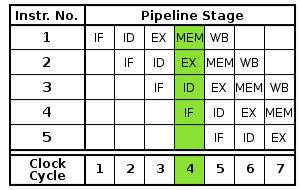
\includegraphics[width=0.5\linewidth]{images/5_stage_pipeline.png}
    \begin{tabular}{|c|c|c|c|c|c|c|c|}
        \toprule
        Instr. No.  & \multicolumn{7}{c|}{Pipeline Stage}                                   \\
        \toprule
        1           & IF                                  & ID & EX & MEM & WB  &     &     \\
        \midrule
        2           &                                     & IF & ID & EX  & MEM & WB  &     \\
        \midrule
        3           &                                     &    & IF & ID  & EX  & MEM &     \\
        \midrule
        4           &                                     &    &    & IF  & ID  & EX  & MEM \\
        \midrule
        5           &                                     &    &    &     & IF  & ID  & EX  \\
        \midrule
        \midrule
        Clock Cycle & 1                                   & 2  & 3  & 4   & 5   & 6   & 7   \\
        \bottomrule
    \end{tabular}
\end{defi}

\begin{defi}[Pipelining]{Taktung}
    % TODO: https://de.wikipedia.org/wiki/Pipeline_(Prozessor)#Taktung (Quelle)
    Je einfacher eine einzelne Stufe aufgebaut ist, desto höher ist die \emph{Frequenz}, mit der sie betrieben werden kann.
    In einer modernen CPU mit einem Kerntakt im Gigahertz-Bereich kann die Befehlspipeline über 30 Stufen lang sein.
    Der \emph{Kerntakt} ist die Zeit, die ein Befehl braucht, um eine Stufe der Pipeline zu durchwandern.
    
    In einer $k$-stufigen Pipeline wird ein Befehl also in $k$ Takten von $k$ Stufen bearbeitet.
    Da in jedem Takt ein neuer Befehl geladen wird, verlässt im Idealfall auch ein Befehl pro Takt die Pipeline.
    
    Der \emph{Takt} wird durch die Zykluszeit der Pipeline bestimmt und berechnet sich aus dem Maximum $\tau_{m}$ aller Stufenverzögerungen $\tau_{i}$ und einem Zusatzaufwand $d$, welcher durch die Zwischenspeicherung der Ergebnisse in Pipeline-Registern verursacht wird.
    
    Die Zykluszeit $\tau$ ist dann definiert durch:
    \[
        \tau = \max_i (\tau_i) + d = \tau_m + d
    \]
\end{defi}

\begin{defi}[Pipelining]{Durchsatz}
    % TODO: https://de.wikipedia.org/wiki/Pipeline_(Prozessor)#Taktung (Quelle)
    Durch das Pipelining wird der \emph{Gesamtdurchsatz} gegenüber Befehlsabarbeitung ohne Pipelining erhöht.
    Die Gesamtzeit für die Pipeline-Verarbeitung mit $k$ Stufen und $n$ Befehlen bei einer Zykluszeit $\tau$ ergibt sich aus:
    \[
        T_k = (k + n - 1) \cdot \tau
    \]
    Erklärung: Anfangs ist die Pipeline leer und wird in $k \cdot \tau$ Schritten gefüllt.
    Nach jeder Stufe wird ein neuer Befehl in die Pipeline geladen, und ein anderer Befehl wird fertiggestellt.
    Die restlichen Befehle werden daher in $(n-1)\cdot \tau$ Schritten fertiggestellt.
\end{defi}

\begin{defi}[Pipelining]{Speedup}
    % TODO: https://de.wikipedia.org/wiki/Pipeline_(Prozessor)#Taktung (Quelle)
    Der bestmögliche \emph{Speedup} beim Pipelining entspricht der Anzahl der Pipeline-Stufen.
    Er wird reduziert durch unausgewogene Ausführungslängen.
    Die Geschwindigkeit der Pipeline ist also direkt beschränkt durch die langsamste Pipeline-Stufe.
    
    Eine effiziente Pipeline-Nutzung setzt voraus, dass eine möglichst hohe Anzahl von Aufträgen (Prozesse) verarbeitet wird.
    Bei nur einem Auftrag entartet die Pipeline zu einer reinen sequentiellen Verarbeitung.
    
    Bildet man nun den Quotienten aus der Gesamtlaufzeit für Befehlsabarbeitung mit und ohne Pipelining, so erhält man den Speedup bei $k$ Stufen und $n$ Befehlen bei einer Zykluszeit $\tau$:
    \[
        S_k = \frac{n \cdot (k \cdot \tau)}{(k + n - 1) \cdot \tau} = \frac{n \cdot k}{k + n - 1}
    \]
\end{defi}

\begin{defi}{Superskalarität}
    Unter \emph{Superskalarität} versteht man die Fähigkeit eines Prozessors, zwei oder mehr skalare Befehle eines Befehlsstroms gleichzeitig mit Hilfe von mehreren parallel arbeitenden Funktionseinheiten auszuführen.
    
    Es handelt sich dabei um eine Nebenläufigkeit bei der Ausführung einzelner Maschinenanweisungen.
    Dazu müssen die parallel abgearbeiten Befehle voneinander unabhängig sein und der Prozessor muss mindestens zwei parallel betreibbare Ausführungseinheiten besitzen.
    
    Superskalarität ermöglicht es, mehr als eine Maschinenanweisung pro Takt zu bearbeiten, während Pipelining die maximal mögliche Taktfrequenz erhöht.
\end{defi}

\begin{defi}{Pipeline-Hazard}
    % TODO: https://de.wikipedia.org/wiki/Pipeline-Hazard (Quelle)
    Alle modernen Prozessoren sind in Pipeline-Architektur ausgeführt:
    Die einzelnen Instruktionen durchlaufen eine mehrstufige Pipeline, in der sie bei jedem Taktzyklus die nächste Stufe erreichen.
    
    Jeder Teilschritt benötigt gewisse Ressourcen des Prozessors (z. B. Datenwege und Rechenwerke) und möglicherweise Ergebnisse einer vorhergegangenen Instruktion.
    Falls eine dieser Ressourcen von einer anderen Instruktion blockiert ist oder Ergebnisse noch nicht zur Verfügung stehen, muss diese Instruktion und alle in der Pipeline folgenden vorübergehend angehalten (\enquote{stalled}) werden.
    
    Die Risiken, den Strom der gleichmäßigen Abarbeitung abreißen zu lassen, nennt man \emph{Pipeline-Hazards}.
\end{defi}

\begin{defi}[Pipeline-Hazard]{Structural Hazards}
    % TODO: https://de.wikipedia.org/wiki/Pipeline-Hazard (Quelle)
    \emph{Structural Hazards} bzw. \emph{Strukturkonflikte} treten auf, wenn Ressourcenkonflikte innerhalb von Befehlen in der Pipeline vorhanden sind, z. B. ein synchroner Zugriff auf einen Registerspeicher mit nur einem Eingang.
    
    Das Beispiel zeigt, dass es sinnvoll ist, voneinander abhängige Befehle möglichst nicht direkt hintereinander auszuführen.
    Moderne Prozessoren können deshalb durch Out-of-Order Execution oder hardwareseitiges Multithreading in vielen Fällen Hazards und Ressourcenkonflikte vermeiden.
\end{defi}

\begin{defi}[Pipeline-Hazard]{Data Hazards}
    % TODO: https://de.wikipedia.org/wiki/Pipeline-Hazard (Quelle)
    \emph{Data Hazards} bzw. \emph{Datenkonflike} ergeben sich aus Datenabhängigkeiten zwischen Befehlen im Programm.
\end{defi}

\begin{defi}{Schleifenparallelisierung}
    % TODO: https://en.wikipedia.org/wiki/Loop_dependence_analysis vlt hilfreich (Quelle)
    TODO
\end{defi}

\begin{defi}{Abhängigkeitsgraph}
    % TODO: https://en.wikipedia.org/wiki/Loop_dependence_analysis vlt hilfreich (Quelle)
    TODO
\end{defi}

\begin{defi}[Pipeline-Hazard]{Control Hazards}
    % TODO: https://de.wikipedia.org/wiki/Pipeline-Hazard (Quelle)
    \emph{Control Hazards} bzw. \emph{Steuerkonflikte} treten bei Instruktionen auf, die den Befehlszähler verändern, z. B. bei bedingten Sprungbefehlen (Branching).
\end{defi}

\begin{defi}{Sprungvorhersage}
    % TODO: https://de.wikipedia.org/wiki/Pipeline-Hazard (Quelle)
    % TODO: https://de.wikipedia.org/wiki/Sprungvorhersage (Quelle)
    Mit der \emph{Predication}-Methode bzw. \emph{Sprungvorhersage} können bestimmte Control Hazards (Branches) aufgelöst werden.
    
    Sie besteht aus den Schritten:
    \begin{enumerate}
        \item Vorhersage, ob ein bedingter Sprung ausgeführt wird
        \item Zieladresse eines Sprunges ermitteln
    \end{enumerate}
\end{defi}

\begin{defi}[Befehlssatzarchitektur]{VLIW}
    % TODO: https://de.wikipedia.org/wiki/Very_Long_Instruction_Word (Quelle)
    \emph{Very Long Instruction Word} (\emph{Very Long Instruction Word}) bezeichnet eine Eigenschaft einer Befehlssatzarchitektur einer Familie von Mikroprozessoren.
    Ziel ist die Beschleunigung der Abarbeitung von sequentiellen Programmen durch Ausnutzung von Parallelität auf Befehlsebene.
    
    Im Gegensatz zu superskalaren Prozessoren werden bei VLIW die Befehle nicht dynamisch zur Laufzeit vom Prozessor den einzelnen Funktionseinheiten zugewiesen, sondern der Compiler gruppiert parallel ausführbare Befehle.
    
    VLIW schließt die Verwendung einer Pipeline-Architektur nicht aus.
    
    TODO: Grafik
\end{defi}

\begin{defi}[Befehlssatzarchitektur]{Explicitly Parallel Instruction Computing (EPIC)}
    Von HP und Intel wurde 1998/99 die Prozessorarchitektur EPIC entworfen und mit dem Intel Itanium ein erster Prozessor realisiert. 
    Die Intel-Version der Architektur wird IA-64 (64 bit) genannt.
    
    EPIC ist die moderne Weiterentwicklung des Konzepts des VLIW.
    
    Hierbei versucht der Compiler, möglichst viele voneinander unabhängige Instruktionen in einer Sequenz zusammenzustellen. 
    Er kann dabei durch Umstellen der Befehle die Reihenfolge innerhalb der Sequenz verändern. Dies darf aber nicht zu anderen Ergebnissen führen!
    Eine solche Sequenz nennt Intel ein \enquote{bundle}.
    
    Das \emph{Explicitly Parallel Instruction Computing} (\emph{EPIC}) bezeichnet ein Programmierparadigma einer Befehlssatzarchitektur.
    Bei der Programmierung von EPIC-CPUs wird die Parallelisierung der Befehle eines Instruktionsstromes explizit vorgenommen.
    
    Die Instruction Set Architecture (ISA) hat Eigenschaften, die die explizite Parallelisierung unterstützen, während eine herkömmliche ISA von einer sequentiellen Abarbeitung der Befehle ausgeht.
    
    Ein Programm, das in einer Nicht-EPIC-Maschinensprache vorliegt, kann auch parallelisiert werden, aber es ist bei der Ausführung eine komplexe Logik notwendig, um parallel ausführbare Instruktionen zu identifizieren, da das Befehlsformat keine Aussagen über parallelisierbare Instruktionen macht.
    
    Eine EPIC-CPU arbeitet nach dem Prinzip der in-order Execution, im Gegensatz zur out-of-order execution der superskalaren CPUs.
\end{defi}

\begin{defi}{Speculative Execution}
    Bei \emph{Speculative Execution} werden untätige Prozessor-Ressourcen verwendet, um für einen potentiellen zukünftigen Stand des Programmflusses Berechnungen vorauszuführen und Ergebnisse bereitzuhalten.
    
    Hier werden in Phasen, in denen der Prozessor nicht voll ausgelastet ist, die folgenden Programmschritte (in der Programmflusszukunft) auf ihre Ausführbarkeit untersucht mit dem Ziel, den wahrscheinlichsten Weg des Programmflusses zu finden.
    Der wahrscheinlichste Ausführungsweg wird verfolgt, und die Ergebnisse werden als \enquote{spekulative Ergebnisse} zwischengespeichert.
    Wenn das Programm an der Stelle angekommen ist, an dem es die Ergebnisse benötigt, stehen sie schon zur Verfügung und es muss nicht auf eine möglicherweise langwierige Berechnung gewartet werden.
    Die zwischengespeicherten Ergebnisse werden ausgelesen und das Passende ausgeführt, die Anderen werden verworfen.
    
    Durch dieses \enquote{Vorausschauen} des Prozessors wird dessen Leistungsfähigkeit auch in Phasen geringerer Auslastung genutzt, um ihn bei hoher Auslastung später zu entlasten.
\end{defi}

\begin{defi}[Speculative Execution]{Control Speculation}
    % http://www.cs.cmu.edu/afs/cs/academic/class/15740-f03/www/lectures/valuepred-slides.pdf
    TODO: Sinnvolle Definition
\end{defi}

\begin{defi}[Speculative Execution]{Data Speculation}
    % http://www.cs.cmu.edu/afs/cs/academic/class/15740-f03/www/lectures/valuepred-slides.pdf
    TODO: Sinnvolle Definition
\end{defi}

\begin{defi}{Attached-Processor-Systeme}
    Eine zusätzliche Einheit,
    die in einer Multiprozessor-Umgebung an die primäre CPU angeschlossen ist.
    Sie arbeitet als Erweiterung der primären CPU und
    nutzt die Systemsoftware und Peripheriegeräte gemeinsam.
\end{defi}
\section{Mehrprozessorsysteme}

\begin{defi}{Flynnsche Klassifikation}
    % https://de.wikipedia.org/wiki/Flynnsche_Klassifikation (Quelle)
    Die \emph{flynnsche Klassifikation}  ist eine Unterteilung von Rechnerarchitekturen, welche 1966 von Michael J. Flynn publiziert wurde.
    Dabei werden die Architekturen nach der Anzahl der vorhandenen Befehls- (Instruction Streams) und Datenströme (Data Streams) unterteilt.
    
    Die vier Kategorien sind:
    \begin{itemize}
        \item \emph{SISD}: Single Instruction, Single Data
              \begin{itemize}
                  \item nicht parallel
                  \item z. B. Von-Neumann-Rechner
              \end{itemize}
        \item \emph{SIMD}: Single Instruction, Multiple Data
              \begin{itemize}
                  \item z. B. Vektor- oder Arrayprozessoren
              \end{itemize}
        \item \emph{MISD}: Multiple Instruction, Single Data
              \begin{itemize}
                  \item irrelevant
              \end{itemize}
        \item \emph{MIMD}: Multiple Instruction, Multiple Data
              \begin{itemize}
                  \item speichergekoppelte Multiprozessoren (Shared Memory)
                  \item nachrichtengekoppelte Multiprozessoren
              \end{itemize}
    \end{itemize}
    
    \centering
    % TODO: https://en.wikipedia.org/wiki/Flynn%27s_taxonomy (Quelle)
    \begin{tabular}{cc}
    \end{tabular}
\end{defi}

\begin{bonus}[Flynn'sche Klassifikation]{Erweiterungen}
    \begin{center}
        \begin{forest}
            for tree={inner sep=2pt,outer sep=0pt,align=center,font=\sffamily\footnotesize,draw}
            [Parallelrechner
                [\emph{SIMD} \\ Single \\ Instruction \\ Multiple \\ Data
                        [Vektor- \\ Prozessoren \\ (auch Mischformen \\ mit MIMD vorhanden!)]
                        [Array- \\ Prozessoren]
                ]
                [\emph{MIMD} \\ Multiple \\ Instruction \\ Multiple \\ Data
                        [Speichergekoppelte \\ Multiprozessoren
                                [Unified \\ Memory \\ Architecture \\ (UMA)]
                                [Non-Uniform \\ Memory \\ Access \\ (NUMA)]
                        ]
                        [Nachrichtengekoppelte \\ Multiprozessoren
                                [Massively \\ Parallel \\ Processing \\ (MPP)]
                                [Cluster Of \\ Workstations \\ (COW)]
                        ]
                ]
            ]
        \end{forest}
    \end{center}
\end{bonus}

\begin{defi}{Shared Memory}
    % TODO: https://de.wikipedia.org/wiki/Shared_Memory (Quelle)
    Bei MIMD-Architekturen unterscheidet man eng gekoppelte und lose gekoppelte Systeme, wobei Mehrprozessorsysteme zur Klasse der eng gekoppelten Systeme gehören.
    In eng gekoppelten Mehrprozessorsystemen teilen sich die verschiedenen Prozessoren einen gemeinsamen Speicher (\emph{Shared Memory}).
    
    Gegenüber lose gekoppelten MIMD-Architekturen hat dies folgende Vorteile:
    \begin{itemize}
        \item die Prozessoren haben alle dieselbe Sicht auf die Daten und können daher auf einfache Art und Weise miteinander kommunizieren
        \item der Zugriff auf den gemeinsamen Speicher erfolgt sehr schnell
    \end{itemize}
    
    Aus diesen Gründen ist ein eng gekoppeltes MIMD-System in der Regel einfacher zu programmieren als ein lose gekoppeltes MIMD-System.
    
    Allerdings kann der gemeinsam genutzte Speicher auch schnell zum Flaschenhals werden, wenn zu viele Prozessoren vorhanden sind, da (bei einem gemeinsam genutzten Speicherbus) zu einer Zeit immer nur ein Prozessor auf den Speicher zugreifen kann.
\end{defi}

\begin{defi}{Speichergekoppelte Systeme}
    Bei speichergekoppelten Multiprozessoren arbeiten alle Prozessoren in einem einheitlichen Adressraum.
    
    Je nach physiklischer Speicherorganisation unterscheidet man:
    \begin{itemize}
        \item \emph{Symmetrische Multiprozessoren (SMP, symmetric multiprocessor)},
              bei denen gleichartige Prozessoren über ein Verbindungsnetzwerk mit einem gemeinsamen Speicher verbunden sind
        \item \emph{Distributed-Shared-Memory Systeme},
              bei denen zwar ein einheitlicher Adressraum existiert,
              aber die Speicher physikalisch auf einzelnen Verarbeitungsknoten verteilt sind
    \end{itemize}
    
    \emph{Bemerkungen:}
    \begin{itemize}
        \item Speichergekoppelte Multiprozessoren gelten als einfacher programmierbar gegenüber nachrichtengekoppelten Multiprozessoren
        \item Nutzbare Parallelität reicht von der Programmebene bis zur Blockebene
        \item Autoparallelisierende Compiler nutzen insbesondere die Parallelisierung der Schleifenebene (einzelne Iterationen nebenläufig abarbeitbar)
    \end{itemize}
\end{defi}

\begin{defi}[Shared Memory]{Uniform Memory Access}
    % TODO: https://de.wikipedia.org/wiki/Uniform_Memory_Access (Quelle)
    \emph{Uniform Memory Access} (\emph{UMA}) steht allgemein für eine Speicherarchitektur in Mehrprozessorsystemen.
    Dabei gibt es nur einen globalen Speicher, auf den von allen Prozessoren aus einheitlich zugegriffen werden kann.
    Im Idealfall jeweils mit derselben Bandbreite und Latenzzeit, weshalb solch ein System auch \emph{Symmetrisches Multiprozessorsystem} (\emph{SMP}) genannt wird.
    
    Das Konzept steht im Gegensatz zu NUMA, bei dem die Zugriffszeit auf den Speicher vom Ort des Speichers abhängen.
    
    TODO: Grafik
\end{defi}

\begin{defi}[Shared Memory]{Non-Uniform Memory Access}
    % TODO: https://de.wikipedia.org/wiki/Non-Uniform_Memory_Access (Quelle)
    \emph{Non-Uniform Memory Access} (\emph{NUMA}) ist eine Computer-Arbeitsspeicher-Architektur für Multiprozessorsysteme, bei denen jeder Prozessor einen eigenen, \enquote{lokalen} Arbeitsspeicher hat, aber anderen Prozessoren über einen gemeinsamen Adressraum \enquote{direkten} Zugriff darauf gewährt (\emph{Distributed Shared Memory}).
    
    Die Speicherzugriffszeiten für eine CPU in einem solchen Verbund hängen daher davon ab, ob sich eine Speicheradresse im CPU-eigenen \enquote{lokalen} oder im \enquote{fremden} Speicher (einer anderen CPU) befindet.
    
    TODO: Grafik
\end{defi}

\begin{defi}{Nachrichtengekoppelte Systeme}
    % TODO: https://pc2.uni-paderborn.de/fileadmin/pc2/lecture_APRS19/VL_APCS.03.pdf (Quelle)
    Beim \emph{nachrichtengekoppelten Multiprozessorsystem} besitzen alle Prozessoren nur räumlich verteilte Speicher und prozessorlokale Adressräume.
    
    Die Kommunikation geschieht durch Austausch von Nachrichten.
    
    TODO: Grafik
\end{defi}

\subsection{Verbindungsnetzwerke}

\begin{defi}{Verbindungsnetzwerk}
    % TODO: https://de.wikipedia.org/wiki/Verbindungsnetzwerk (Quelle)
    Das \emph{Verbindungsnetzwerk} ermöglicht den Datenaustausch und die Verteilung des Programms zwischen den Prozessoren.
    
    Um einen hohen Datentransfer zu erhalten, wird eine große Anzahl von physischen Verbindungen benötigt.
\end{defi}

\begin{defi}[Verbindungsnetzwerk]{Topologie}
    % TODO: https://de.wikipedia.org/wiki/Verbindungsnetzwerk (Quelle)
    % TODO: https://de.wikipedia.org/wiki/Topologie_(Rechnernetz) (Quelle)
    Die \emph{Topologie} ist der wesentlichste Parameter eines Verbindungsnetzwerkes.
    Sie ist verantwortlich für die fundamentalen Merkmale und Begrenzungen des Verbindungsnetzwerkes.
    
    Die Topologie eines Rechnernetzes beschreibt die spezifische Anordnung der Geräte und Leitungen, die ein Rechnernetz bilden, über das die Computer untereinander verbunden sind und Daten austauschen.
    
    Topologien werden grafisch (nach der Graphentheorie) mit Knoten und Kanten dargestellt.
    Dabei sind Knoten die Kommunikationsteilnehmer des Netzwerkes und Kanten die physikalischen oder logischen Verbindungen.
\end{defi}

\begin{defi}[Verbindungsnetzwerk]{Latenz}
    Die \emph{Latenz} eines Verbindungsnetzwerkes gibt die Zeit für den Transfer zwischen den Knoten an.
\end{defi}

\begin{defi}[Verbindungsnetzwerk]{Bandbreite}
    Die \emph{Bandbreite} eines Verbindungsnetzwerkes gibt das Verhältnis der transferierten Daten zur Zeit an.
\end{defi}

\begin{defi}[Verbindungsnetzwerk]{Durchmesser}
    % TODO: https://de.wikipedia.org/wiki/Topologie_(Rechnernetz) (Quelle)
    Der \emph{Durchmesser} einer Topologie bzw. eines Verbindungsnetzwerkes beschreibt die maximale direkte Entfernung zwischen zwei Knoten in Hops.
    
    Damit ist er ein direktes Maß für die zu erwartenden maximalen Transferzeiten, d. h. je größer der Durchmesser, desto größer die Transferzeit im ungünstigsten Fall.
\end{defi}

\subsubsection{Statische Verbindungsnetzwerke}

\begin{defi}{Statisches Verbindungsnetzwerk}
    % TODO: https://de.wikipedia.org/wiki/Verbindungsnetzwerk (Quelle)
    \emph{Statische Verbindungsnetzwerke} sind fest verdrahtet.
    Jeder Knoten besitzt eine feste Anzahl von Nachbarn nebst entsprechenden direkten Verbindungen (Links) zu ihnen.
    
    Das Netzwerk selbst besteht nur aus den Leitungen, besitzt also keinerlei Vermittlungsfunktion.
    Diese wird indirekt über die beteiligten Knoten ausgeführt.
    
    Netze dieser Art sind einmal aufgebaut nicht rekonfigurierbar.
    Beispiele für statische Verbindungsnetzwerke sind Gitter oder Ringe, Bäume und Hypercubes
\end{defi}

\begin{defi}[Statisches Verbindungsnetzwerk]{Lineare Anordnung}
    \begin{center}
        \begin{tikzpicture}
            \foreach \x in {0,...,5} {
                    \node[circle, draw=blue, fill=blue] (\x0) at (\x, 0) {};
                }
            
            \foreach \x [remember=\x as \lastx (initially 0)] in {1,...,5} {
                    \draw (\lastx0) to[] node[left]{}(\x0);
                }
        \end{tikzpicture}
        \\
        Diameter = $N-1$
    \end{center}
\end{defi}

\begin{defi}[Statisches Verbindungsnetzwerk]{Ring}
    \begin{center}
        \begin{tikzpicture}
            \node[circle, draw=blue, fill=blue] (d0) at (0, 0) {};
            \node[circle, draw=blue, fill=blue] (d1) at (0, 1) {};
            \node[circle, draw=blue, fill=blue] (d2) at (1, 1) {};
            \node[circle, draw=blue, fill=blue] (d3) at (1, 0) {};
            \draw (d0) to[bend left] node[left]{}(d1);
            \draw (d1) to[bend left] node[left]{}(d2);
            \draw (d2) to[bend left] node[left]{}(d3);
            \draw (d3) to[bend left] node[left]{}(d0);
        \end{tikzpicture}
        \\
        Diameter = $\frac{N}{2}$
    \end{center}
\end{defi}

\begin{defi}[Statisches Verbindungsnetzwerk]{Torus}
    2D-Torus:
    \begin{center}
        \begin{tikzpicture}[circlestyle/.style={circle, draw=blue, fill=blue}]
            \foreach \x in {0, ..., 5} {
                    \foreach \y in {0, ..., 5} {
                            \node[circlestyle] (\x\y) at (\x, \y) {};
                        }
                }
            
            \foreach \x in {0,...,5}{
                    \foreach \y [count=\yi] in {0,...,4}{
                            \draw (\x\y)--(\x\yi) (\y\x)--(\yi\x);
                        }
                }
            
            \foreach \x in {0,...,5} {
                    \draw (\x0) to[bend left] node[left]{}(\x5);
                }
            \foreach \y in {0,...,5}{
                    \draw (0\y) to[bend left] node[left]{}(5\y);
                }
        \end{tikzpicture}
        \\
        Diameter = $\sqrt{N}$
    \end{center}
\end{defi}

\begin{defi}[Statisches Verbindungsnetzwerk]{Gitter}
    2D-Gitter:\\
    \begin{center}
        \begin{tikzpicture}[circlestyle/.style={circle, draw=blue, fill=blue}]
            \foreach \x in {0, ..., 5}{
                    \foreach \y in {0, ..., 5}{
                            \node[circlestyle] (\x\y) at (\x, \y) {};
                        }
                }
            
            \foreach \x in {0,...,5}{
                    \foreach \y [count=\yi] in {0,...,4}{
                            \draw (\x\y)--(\x\yi) (\y\x)--(\yi\x);
                        }
                }
        \end{tikzpicture}
        \\
        Diameter = $2\cdot\left(\sqrt{N} - 1\right)$
    \end{center}
\end{defi}

\begin{defi}[Statisches Verbindungsnetzwerk]{Hypercube}
    \begin{itemize}
        \item Anzahl der Knoten: $N = 2d$
        \item Diameter: $d = \log_2 N$
        \item Greycode Adressierung: Jeder Knoten verbunden mit $d$ anderen Knoten unterscheidet sich durch \emph{ein Bit} in der Adresse
        \item Beispiele: Intel iPSC und NCUBE
    \end{itemize}
    \tcblower
    \begin{center}
        \begin{tabular}{@{}cccc@{}}
            \begin{tikzpicture}[circlestyle/.style={circle, draw=blue, fill=blue}]
                \node[circlestyle] (A) at (0,0) {};
            \end{tikzpicture} & 
            \begin{tikzpicture}[circlestyle/.style={circle, draw=blue, fill=blue}]
                \node[circlestyle] (A) at (0,0) {};
                \node[circlestyle] (B) at (1,0) {};
                \draw (A) -- (B);
            \end{tikzpicture} & 
            \begin{tikzpicture}[circlestyle/.style={circle, draw=blue, fill=blue}]
                \node[circlestyle] (A) at (0,0) {};
                \node[circlestyle] (B) at (1,0) {};
                \draw (A) -- (B);
                
                \node[circlestyle] (C) at (0.5, 0.5) {};
                \node[circlestyle] (D) at (1.5, 0.5) {};
                \draw (C) -- (D);
                
                \draw (A) -- (C);
                \draw (B) -- (D);
            \end{tikzpicture} & 
            TODO: tikzpicture                         \\
            0d                         & 1d & 2d & 4d \\
        \end{tabular}
    \end{center}
\end{defi}

\begin{defi}[Statisches Verbindungsnetzwerk]{Baum}
    % TODO: https://de.wikipedia.org/wiki/Topologie_(Rechnernetz) (Quelle)
    \emph{Baum-Topologien} sind dadurch gekennzeichnet, dass sie eine Wurzel (der erste bzw. obere Knoten) haben, von der eine oder mehrere Kanten (Links) ausgehen.
    Diese führen weiterhin zu einem Blatt (Endknoten) oder \enquote{rekursiv} zu inneren Knoten von Teilbäumen.
    \tcblower
    \begin{center}
        \begin{tabular}{@{}cc@{}}
            Planares Layout & Fetter Baum \\
            \begin{tikzpicture}[circlestyle/.style={circle, draw=blue, fill=blue}]
                \foreach \y in {0, ..., 3}{
                        \node[circlestyle] (0\y) at (0,\y) {};
                        \node[circlestyle] (1\y) at (1,\y) {};
                        \node[circlestyle] (3\y) at (3,\y) {};
                        \node[circlestyle] (4\y) at (4,\y) {};
                    }
                % Connections between nodes
                \draw (00) -- (01);
                \draw (10) -- (11);
                \draw (30) -- (31);
                \draw (40) -- (41);
                
                \draw (02) -- (03);
                \draw (12) -- (13);
                \draw (32) -- (33);
                \draw (42) -- (43);
                %%%
                % Connections between connections
                \draw (0, 0.5) -- (1, 0.5);
                \draw (3, 0.5) -- (4, 0.5);
                
                \draw (0, 2.5) -- (1, 2.5);
                \draw (3, 2.5) -- (4, 2.5);
                
                \draw (0.5, 0.5) -- (0.5, 2.5);
                \draw (3.5, 0.5) -- (3.5, 2.5);
                
                \draw (0.5, 1.5) -- (3.5, 1.5);
                %%%
            \end{tikzpicture}
                            & 
            \begin{tikzpicture}[circlestyle/.style={circle, draw=blue, fill=blue}]
                \foreach \y in {0, ..., 3}{
                        \node[circlestyle] (0\y) at (0,\y) {};
                        \node[circlestyle] (1\y) at (1,\y) {};
                        \node[circlestyle] (3\y) at (3,\y) {};
                        \node[circlestyle] (4\y) at (4,\y) {};
                    }
                % Connections between nodes
                \draw (00) -- (01);
                \draw (10) -- (11);
                \draw (30) -- (31);
                \draw (40) -- (41);
                
                \draw (02) -- (03);
                \draw (12) -- (13);
                \draw (32) -- (33);
                \draw (42) -- (43);
                %%%
                % Connections between connections
                \draw (0, 0.4) -- (1, 0.4);
                \draw (0, 0.5) -- (1, 0.5);
                \draw (0, 0.6) -- (1, 0.6);
                
                \draw (3, 0.4) -- (4, 0.4);
                \draw (3, 0.5) -- (4, 0.5);
                \draw (3, 0.6) -- (4, 0.6);
                
                \draw (0, 2.4) -- (1, 2.4);
                \draw (0, 2.5) -- (1, 2.5);
                \draw (0, 2.6) -- (1, 2.6);
                
                \draw (3, 2.4) -- (4, 2.4);
                \draw (3, 2.5) -- (4, 2.5);
                \draw (3, 2.6) -- (4, 2.6);
                
                \draw (0.4, 0.4) -- (0.4, 2.6);
                \draw (0.5, 0.4) -- (0.5, 2.6);
                \draw (0.6, 0.4) -- (0.6, 2.6);
                
                \draw (3.4, 0.4) -- (3.4, 2.6);
                \draw (3.5, 0.4) -- (3.5, 2.6);
                \draw (3.6, 0.4) -- (3.6, 2.6);
                
                \draw (0.4, 1.4) -- (3.6, 1.4);
                \draw (0.4, 1.5) -- (3.6, 1.5);
                \draw (0.4, 1.6) -- (3.6, 1.6);
                %%%
            \end{tikzpicture}
        \end{tabular}

        Diameter = $\log_2 N$
    \end{center}
\end{defi}

\begin{bonus}{Übersicht statischer Verbindungsnetzwerke}
    \begin{tabularx}{\textwidth}{@{}lXXX@{}}
        \toprule
        Topologie          & Anzahl der Verbindungskanäle pro Knoten & Maximale Entfernung (Diameter) & Gesamtanzahl der Verbindungskanäle \\
        \midrule
        Ring               & 2                                       & $\frac{N}{2}$                  & $N-1$                              \\
        Baum               & 3                                       & $2\cdot (\log_2 N - 1)$        & $N-1$                              \\
        2D - Gitter        & 4                                       & $2\cdot \sqrt{N}$              & $2\cdot N$                         \\
        3D - Gitter        & 6                                       & $3\cdot \sqrt[3]{N}$           & $3\cdot N$                         \\
        Hexagon. Gitter    & 6                                       & $3\cdot \sqrt[3]{N}$           & $3\cdot N$                         \\
        Hypercube          & $\log_2 N$                              & $\log_2 N$                     & $N \log_2 \frac{N}{2}$             \\
        Vollst. Vernetzung & $N - 1$                                 & 1                              & $N \cdot \frac{N-1}{2}$            \\
    \end{tabularx}
\end{bonus}

\subsubsection{Dynamische Verbindungsnetzwerke}

\begin{defi}{Dynamisches Verbindungsnetzwerk}
    % TODO: https://de.wikipedia.org/wiki/Verbindungsnetzwerk (Quelle)
    \emph{Dynamische Verbindungsnetzwerke} zeichnen sich dadurch aus, dass die Verbindungen zwischen den Knoten über zum Netz gehörende Koppelelemente realisiert werden.
    
    Dabei können diese Koppelelemente in mehreren Stufen hintereinander angeordnet sein, weshalb man diese Art der Verbindungsnetzwerke nochmals in einstufige und mehrstufige Netze unterteilt.
    Eine Stufe enthält dabei eine gewisse Anzahl Koppelelemente.
    
    Genauer gesagt sorgt das Netz dafür, dass Senderknoten mittels einer Permutationsfunktion auf Empfängerknoten geschaltet werden.
    Dabei können entweder alle $n!$ Permutationen geschaltet werden, oder nur einige.
\end{defi}

\begin{defi}[Dynamisches Verbindungsnetzwerk]{Bus}
    % TODO: https://de.wikipedia.org/wiki/Verbindungsnetzwerk (Quelle)
    Bei einer \emph{Bus-Topologie} sind alle Geräte direkt mit demselben Übertragungsmedium, dem Bus verbunden.
    Es gibt keine aktiven Komponenten zwischen den Geräten und dem Medium.
    
    Durch die wahlweise Zuschaltung einzelner Verarbeitungsknoten zum Datentransfer an einen Bus ist das Bussystem eine typische dynamische Verbindungseinrichtung.
    
    Der Bus bildet die Engstelle im busgekoppelten Multiprozessorsystem, so dass auch Doppelbusse oder allgemein Mehrfachbusse eingesetzt werden.
\end{defi}

\begin{defi}{Crossbar}
    \begin{itemize}
        \item $M \times M$ Matrix
        \item einfaches Weiterleiten an mehrere Ausgänge
        \item komplexe Steuerung
        \item Verdrahtungsaufwand
        \item Pufferung bei Blockierungen
        \item Diameter = 1, d. h. beliebige Verbindungen können unter Einsatz jeweils nur einer Schaltzelle realisiert werden
    \end{itemize}
\end{defi}

\begin{defi}{Zellenbasierte Systeme}
    Zellen mit 2 Eingängen und 2 Ausgägen bilden die Basis für solche Systeme.
    \begin{itemize}
        \item 2 Bit $\to$ 4 Schaltzustände
        \item gerade Zellen
        \item kreuzende Zellen
        \item Eingänge mit mehreren Ausgängen verbunden (seltener genutzt)
    \end{itemize}
\end{defi}

\begin{defi}[Dynamisches Verbindungsnetzwerk]{Einstufiges Netzwerk}
    % TODO: https://de.wikipedia.org/wiki/Verbindungsnetzwerk (Quelle)
    \emph{Einstufige dynamische Verbindungsnetzwerke} bestehen aus nur einer so genannten Stufe von Schaltzellen beziehungsweise nur aus der Schaltzelle selbst.
    
    Die Zellen sind in der Regel eine mehr oder weniger komplexe Form eines Kreuzschienenverteilers (Crossbar), der selbst schon ein einstufiges dynamisches Verbindungsnetzwerk darstellt.
    
    TODO: Grafik
\end{defi}

\begin{defi}[Dynamisches Verbindungsnetzwerk]{Mehrstufiges Netzwerk}
    \emph{Mehrstufige dynamische Verbindungsnetzwerke} zeichnen sich dadurch aus, dass mehrere Stufen von Schaltzellen hintereinander geschaltet werden.
    Zwischen den Stufen besteht eine feste Verdrahtung.
    
    TODO: Grafik
\end{defi}

\begin{defi}{Omega-Netzwerk}
    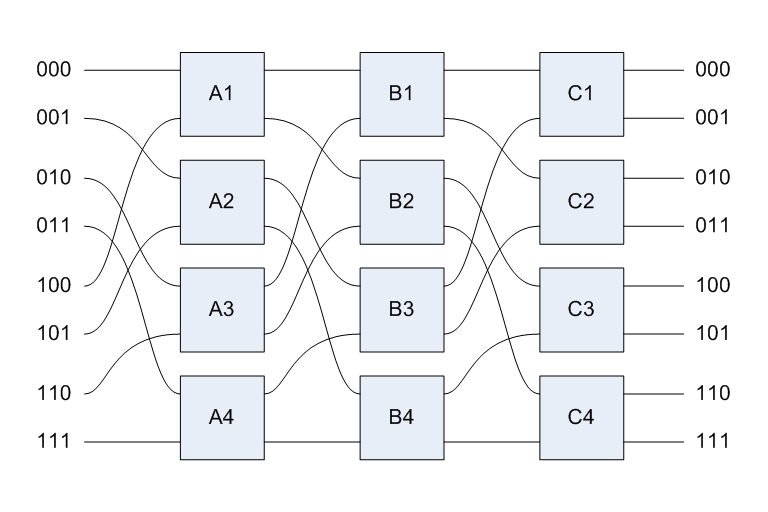
\includegraphics[width=\textwidth]{images/OmegaNetwork.jpg}
    % TODO: By Bjmyers17, CC BY-SA 3.0, \url{https://commons.wikimedia.org/w/index.php?curid=75639225}
\end{defi}

\begin{defi}[Dynamisches Verbindungsnetzwerk]{Zelle}
    Die \emph{Zell-Topologie} kommt hauptsächlich bei drahtlosen Netzen zum Einsatz.
    
    Eine Zelle ist der Bereich um eine Basisstation (z. B. Wireless Access Point), 
    in dem eine Kommunikation zwischen den Endgeräten und der Basisstation möglich ist.
    Innerhalb einer Zelle entspricht die Zell-Topologie der Bus-Topologie.
\end{defi}

\begin{defi}{Benes-Netzwerk}
    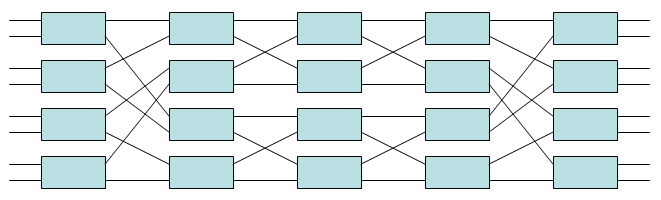
\includegraphics[width=\textwidth]{images/Benesnetwork.png}
    % TODO: By Piggly - Own work, Public Domain, \url{https://commons.wikimedia.org/w/index.php?curid=2988080}
\end{defi}

\subsubsection{Cluster-Interconnects}

\begin{defi}{Cluster-Interconnect}
    % TODO: https://de.wikipedia.org/wiki/Cluster_Interconnect (Quelle)
    Der \emph{Cluster-Interconnect} ist eine Verbindung zwischen den Cluster-Membern, über die alle Arten von relevanten Daten ausgetauscht werden.
    
    Sie wird in aller Regel als privates Netzwerksegment konzipiert, um höchstmögliche Betriebssicherheit zu gewährleisten oder auch andere Netzwerkarchitekturen abbilden zu können;
    denn diese Zwischenverbindung ist -- in Abhängigkeit von der Größe des Clusters -- mit möglichst geringer Latenz und hoher Übertragungsrate auszustatten, um keinen Flaschenhals zu schaffen.
    
    Dazu häufig verwendete Technologien sind Gigabit-Ethernet oder auch das teurere InfiniBand.
\end{defi}

\begin{defi}[Cluster-Interconnect]{InfiniBand}
    % TODO: https://de.wikipedia.org/wiki/InfiniBand (Quelle)
    \emph{InfiniBand} ist eine Spezifikation einer Hardwareschnittstelle zur seriellen Hochgeschwindigkeitsübertragung auf kurzen Distanzen mit geringer Latenz.
    
    Sie wird bevorzugt in Rechenzentren verwendet, beispielsweise für die Verbindungen der Server in Computerclustern untereinander und zur Verbindung zwischen Servern und benachbarten Massenspeichersystemen wie Storage Area Networks (SAN).
    
    InfiniBand benutzt bidirektionale Punkt-zu-Punkt-Verbindungen zur latenzarmen Datenübertragung mit Verzögerungszeiten unter \SI{2}{\micro\second}, und erreicht theoretische Datenübertragungsraten pro Kanal zwischen \SI{2,5}{\giga\bit\per\second} (SDR) und \SI{50}{\giga\bit\per\second} (HDR) in beide Richtungen.
    Bei InfiniBand können mehrere Kanäle zur Skalierung in einem Kabel transparent gebündelt werden.
\end{defi}

\begin{defi}[Cluster-Interconnect]{Gigabit Ethernet}
    Gigabit Ethernet \ldots
    \begin{itemize}[\ldots]
        \item wird vorwiegend in lokalen Netzwerken genutzt,
              auch für Heimanwender mit RJ45 Stecker für Kupferkabel (z.B. Lan-Buchsen am Router)
        \item ist für Glasfaser und (twisted-pair) Kupferkabel spezifiziert,
              höhrere Bandbreiten aber nur über Glasfaser umsetzbar: bis zu 100 Gb/s
        \item ist Switch-basiert und abwärtskompatibel
        \item nutzt spezielle Kollisionserkennung / -vermeidung,
              wie CSMA / CD (Carrier Sense Multiple Access with Collision Detection)
    \end{itemize}
\end{defi}

\begin{defi}[Verbindungsnetzwerk]{Klassifikation}
    \begin{center}
        \begin{forest}
            for tree={inner sep=2pt,outer sep=0pt,align=center,font=\sffamily\footnotesize,draw}
            [Verbindungsnetzwerk
                [statisch
                        [ein-\\dimensional]
                        [zwei-\\dimensional]
                        [mehr-\\dimensional]
                ]
                [dynamisch
                        [Bussysteme]
                        [Zellenbasierte \\ Netze
                                [einstufig]
                                [mehrstufig
                                        [blockierend]
                                        [nicht-blockierend]
                                ]
                        ]
                        [Kreuzschienenverteiler \\ (Crossbars)]
                ]
            ]
        \end{forest}
    \end{center}
\end{defi}

\subsection{Cache-Kohärenz}
\begin{defi}{Cache-Kohärenz}
    \begin{itemize}
        \item wichtig bei Mehrprozessorsystemen mit Shared-Memory oder Shared Virtual Memory $\to$ SMP
        \item Maßnahmen zur Verhinderung von unterschiedlichen Versionen der gleichen Cache-Zeile in 2 oder mehreren Caches
        \item Technische Lösungen:
              \begin{itemize}
                  \item \emph{Snooping Caches} (auf den Leitungen den Datenverkehr ausschnüffeln == to snoop) $\to$ Bus-basierte Systeme
                  \item \emph{Directory-basierte Caches} $\to$ komplexere Verbindungsnetze
              \end{itemize}
    \end{itemize}
\end{defi}

\begin{defi}[Cache-Kohärenz]{Snooping Cache Protocols}
    Es gibt mehrere Snoopy-Protokolle (z.B. MESI).
    Sie basieren auf der \enquote{Invalidate}-Strategie:
    \begin{itemize}
        \item beim Schreiben von \enquote{shared data} wird ein \enquote{invalidate}-Signal an alle anderen Caches gesendet,
              die eine Kopie dieses Datums als ungültig kennzeichnen
        \item beim Lesen kann jeder Prozessor seine gültige Version der Cache-Zeile verwenden
        \item findet ein Prozessor beim Lesen kein gültiges Datum: Read-Miss
              \begin{itemize}
                  \item bei \enquote{write-through}-Caches befindet sich das Memory immer im aktuellen Zustand:
                        Datum wird in den anfordernden Cache gelesen
                  \item bei \enquote{write-back}-Caches:
                        suche (snoop) in den anderen Caches nach einer gültigen Version
              \end{itemize}
    \end{itemize}
\end{defi}

\begin{defi}[Cache-Kohärenz]{Directory-basierte Caches}
    Bus-basierte Snooping-Protokolle skalieren nicht bei großen Netzwerken mit NUMA-Architektur
    $\to$ Directory-Protokolle $\to$ ccNUMA \\
    Directory-basierte Protokolle sind ähnlich zu Snoopy-Protokoll.
    Das Directory hat ein Zustandsfeld mit 3 möglichen Zuständen:
    \begin{itemize}
        \item \emph{Shared:}     $\geq$ 1 Prozessor besitzen Daten, Memory aktuell
        \item \emph{Uncached:}   Kein Prozessor (kein Cache) besitzt gültige Daten
        \item \emph{Exclusive:}  1 Prozessor (owner) besitzt die Daten, Memory nicht aktuell
    \end{itemize}
\end{defi}

\subsection{Aufgaben}

\begin{aufgabe}{Multiprozessoren}
    Nennen Sie zwei verschiedene Arten von nachrichtengekoppelten Multiprozessoren.
    \tcblower
    \begin{itemize}
        \item Massively Parallel Processor (MPP)
        \item Cluster Of Workstation (COW)
    \end{itemize}
\end{aufgabe}

\begin{aufgabe}{Multiprozessoren}
    Welche beiden Arten von speichergekoppelten Multiprozessor-Systemen wurden in der Vorlesung unterschieden?
    \tcblower
    \begin{itemize}
        \item Uniform Memory Access (UMA)
        \item Non Uniform Memory Access (NUMA)
    \end{itemize}
\end{aufgabe}

\begin{aufgabe}{Multiprozessoren}
    Zwischen welchen speichergekoppelten Multiprozessoren unterscheidet man je nach physikalischer Speicherorganisation?
    \tcblower
    \begin{itemize}
        \item Symmetric multiprocessor (SMP)
        \item Distributed shared memory Systeme
    \end{itemize}
\end{aufgabe}

\begin{aufgabe}{Distributed Memory Machines}
    Auf welche beiden Arten kann eine Distributed Memory Machine realisiert werden?
    \tcblower
    \begin{itemize}
        \item speichergekoppelt als shared virtual memory (SVM) $\to$ NUMA
        \item nachrichtengekoppelt (z.B. Cray T3E)
    \end{itemize}
\end{aufgabe}

\begin{aufgabe}{Verbindungsnetzwerk}
    Nennen und erklären Sie kurz die fünf grundlegenden Eigenschaften eines Verbindungsnetzwerkes.
    \tcblower
    \begin{tabularx}{\textwidth}{@{}lX@{}}
        \toprule
        Eigenschaft            & Erklärung                                                                                                                                           \\
        \midrule
        Latenz (latency)       & Zeit für den Transfer zwischen den Knoten                                                                                                           \\
        Bandbreite (bandwidth) & $\frac{\text{transferierte Daten}}{Zeit}$, Bandbreite eines Link: $\text{bw} = \omega \cdot \frac{1}{t} \left(\frac{\text{bit}}{\text{sec}}\right)$ \\
        Diameter               & maximale Distanz zwischen zwei beliebigen Prozessoren                                                                                               \\
        Topologie              & wie sind die Nachbarknoten angeordnet und erreichbar                                                                                                \\
        \multicolumn{2}{@{}l@{}}{Statische oder dynamische Leitungswege}
    \end{tabularx}
\end{aufgabe}

\begin{aufgabe}{Verbindungsnetzwerk}
    Nennen Sie drei unterschiedliche Verbindungsnetzwerk-Topologien.
    \tcblower
    \begin{itemize}
        \item Torus
        \item (Hyper)cube / Mesh
        \item Tree / Fat Tree
    \end{itemize}
\end{aufgabe}

\begin{aufgabe}{Verbindungsnetzwerk}
    Durch welche physikalische Maßnahme kann bei einem Tree-Netzwerk der Durchsatz erhöht werden?
    \tcblower
    Man erstellt eine zunehmende Anzahl an Leitungen zur Wurzel hin ($\to$ Fat Tree).
\end{aufgabe}

\begin{aufgabe}{Verbindungsnetzwerk}
    Wie groß ist der Durchmesser eines 2D Torus mit N Gitterpunkten?
    \tcblower
    $$\sqrt{N}$$
\end{aufgabe}

\begin{aufgabe}{Verbindungsnetzwerk}
    Was sind die zwei gebräuchlichsten Netzwerktypen im HPC-Bereich?
    \tcblower
    \begin{itemize}
        \item Gbit Ethernet
        \item Infiniband
    \end{itemize}
\end{aufgabe}

\begin{aufgabe}{Cache-Kohärenz}
    Bei Mehrprozessorsystemen mit welchem Speicher ist Cache-Kohärenz wichtig?
    \tcblower
    \begin{itemize}
        \item Shared Memory
        \item Shared Virtual Memory
    \end{itemize}
\end{aufgabe}

\begin{aufgabe}{Cache-Kohärenz}
    Geben Sie zwei technische Lösungen an, um Cache-Kohärenz herzustellen.
    \tcblower
    \begin{itemize}
        \item Snooping Caches
        \item Directory-basierte Systeme
    \end{itemize}
\end{aufgabe}

\begin{aufgabe}{Cache-Kohärenz}
    Durch welches Hilfsmittel kann in Bus-basierten Systemen mit \enquote{write-back}-Caches Cache-Kohärenz realisiert werden?
    \tcblower
    Snoopy-Protokolle
\end{aufgabe}

\begin{aufgabe}{Cache-Kohärenz}
    Auf welcher Strategie basieren Snoopy-Protokolle?
    \tcblower
    Invalidate Strategie
\end{aufgabe}

\begin{aufgabe}{Cache-Kohärenz}
    Womit lässt sich Cache-Kohärenz bei Distributed Memory Systemen realisieren?
    \tcblower
    Directory basierte Protokolle
\end{aufgabe}

\begin{aufgabe}{Cache-Kohärenz}
    Wie lauten die drei möglichen Zustände des Zustandsfeldes der Directory bei einem Directory-basierten Protokoll?
    \tcblower
    \begin{itemize}
        \item \emph{Shared:}     $\geq$ 1 Prozessor besitzen Daten, Memory aktuell
        \item \emph{Uncached:}   Kein Prozessor (kein Cache) besitzt gültige Daten
        \item \emph{Exclusive:}  1 Prozessor (owner) besitzt die Daten, Memory nicht aktuell
    \end{itemize}
\end{aufgabe}
\section{Multithreading}

\begin{defi}{Thread}
    Ein Thread ist \ldots
    \begin{itemize}[\ldots]
        \item ein Stück Code zusammen mit einem Zustand,
              gespeichert in:
              \begin{itemize}
                  \item Register File
                  \item Stack
                  \item Program pointer
              \end{itemize}
        \item eine \enquote{leichtgewichtige} Einheit für den Ablauf von Befehlen (light-weight)
        \item in vielen Betriebssystemen die kleinste Einheit,
              die verwaltet (schedule) werden kann.
        \item die Basis für ein Programmiermodell bei parallelen Rechnern (SMP-Rechner: OpenMP).
    \end{itemize}
\end{defi}

\begin{defi}{Multithreading}
    \emph{Multithreading} beschreibt viele \enquote{gleichzeitig} verwaltbare und ablaufbare Threads bei \ldots
    \begin{itemize}[\ldots]
        \item gleichzeitig bearbeiteten Programmen (multi-programming)
        \item einem parallelen Programm
        \item verschiedenen, in der Regel unabhängigen, Teilen eines sequentiellen Programms,
              z. B. verschiedene Iterationen einer Schleife
    \end{itemize}
\end{defi}

\begin{defi}{Task vs Thread}
    \emph{Process = Task} $\neq$ \emph{Thread}
    \begin{itemize}
        \item Ein Task enthält mindestens einen Thread
        \item Multiple Threads können \enquote{gleichzeitig} in einem Prozessor bearbeitet werden
        \item Tasks besitzen unabhängige Adressräume (address spaces),
              wohingegen Threads einen Adressraum eines Tasks gemeinsam nutzen
              \begin{itemize}
                  \item \underline{Vorteil:} Die gemeinsame Nutzung des Adressraums führt zu einem schnelleren \enquote{context switch}
                        (Umschalten des Prozessors von einem Thread zum anderen)
                  \item \underline{Nachteil:} Multithreading erfordert Synchronisation für den Zugriff auf globale Daten
              \end{itemize}
    \end{itemize}
\end{defi}

\begin{example}{Threads Anwendung und Einsatz}
    Anwendungen für Threads:
    \begin{itemize}
        \item Web-Server: ein Thread für eine Anfrage
        \item Router: ein Thread für ein Paket
        \item Vordergrund / Hintergrund: ein Thread für ein GUI,
              ein anderer zur Berechnung der Aufgabe
    \end{itemize}
    Library:
    \begin{itemize}
        \item Pthreads (nach einem POSIX-Standard)
        \item Routinen für
              \begin{itemize}
                  \item Thread-Erzeugung, Beendigung
                  \item Wechselseitiger Ausschluss und Semaphoren zur Synchronisation
              \end{itemize}
    \end{itemize}
\end{example}

\begin{defi}[Threads]{Simultaneous Multithreading (SMT)}
    Bei Einprozessor-Systemen: \\
    \begin{tabularx}{\textwidth}{|lX|}
        \toprule
        Fakt:    & Superskalare und VLIW Prozessoren holen (fetch) und führen (execute) mehrere Befehle pro Clock Cycle aus \\
        \midrule
        Problem: & Ein einzelner Thread besitzt nicht genug \enquote{instruction-level parallelism}                         \\
        \midrule
        Lösung:  & Ausführen der Befehle von vielen parallelen Threads in einem Clock Cycle                                 \\
        \midrule
        Vorteil: & Die Leistung (performance) der einzelnen Threads wird nicht von anderen Threads beeinträchtigt           \\
        \bottomrule
    \end{tabularx}
    \\
    $\to$ bei Intel wird SMT \enquote{Hyper-threading} genannt.
\end{defi}

\section{Aufgaben}

\begin{aufgabe}{Multithreading}
    Was ist ein Thread?
    \tcblower
    Ein Thread \ldots
    \begin{itemize}[$\ldots$]
        \item ist ein Stück Code zusammen mit einem Zustand, gespeichert in:
              \begin{itemize}
                  \item Register File
                  \item Stack
                  \item Program pointer
              \end{itemize}
        \item ist eine \enquote{leichtgewichtige} Einheit für den Ablauf von Befehlen (light-weight)
        \item ist in vielen Betriebssystemen die kleinste Einheit, die verwaltet (schedule) werden kann
        \item bildet die Basis für ein Programmiermodell bei parallelen Rechnern (SMP-Rechner: OpenMP)
    \end{itemize}
\end{aufgabe}

\begin{aufgabe}{Multithreading}
    Wodurch unterscheidet sich ein Task (Prozess) von einem Thread?
    \tcblower
    \begin{itemize}
        \item Ein Prozess enthält mindestens einen Thread
        \item Multiple Threads können \enquote{gleichzeitig} in einem Prozessor bearbeitet werden
        \item Prozesse besitzen unabhängige Adressräume (address spaces), wohingegen Threads einen Adressraum eines Prozesses gemeinsam nutzen
    \end{itemize}
\end{aufgabe}
\section{Vektorrechner}

\begin{defi}[Vektorprozessoren]{Idee}
    Mathematisch-technische Anwendungen lassen sich erheblich in der Ausführung beschleunigen,
    wenn für Vektoroperationen:
    \begin{itemize}
        \item Spezielle, schnelle Hardware zur Verfügung steht und
        \item in der Programmiersprache Konstrukte zur Beschreibung von Vektor-Operationen verhanden sind
              (HPC Fortran, und zum Teil auch Fortran 90) oder
        \item der Compiler automatisch Programmteile als vektorisierbar erkennt
              (zum Teil mit Hilfe von Direktiven)
    \end{itemize}
    Mögliche Operationen (meist beschränkt auf Floating Point):
    \begin{itemize}
        \item $v = v \pm v, v = s \pm v$
        \item $v = v \cdot v, v = s \cdot v$
        \item mit n-elementigem Vektor $v$ und Skalar $s$
    \end{itemize}
    Eine Division wurde zunächst mit Hilfe einer Reziprok-Funktionseinheit berechnet:
    $v = \frac{1.0}{v}$
\end{defi}

\begin{defi}[Vektorprozessoren]{Ziel}
    Mit (im Idealfall!) einer Vektoroperation können gleichzeitig alle Elemente von zwei Vektoren verknüpft werden:
    \begin{align*}
        vc[1] & = va[1] \pm vb[1] \\
        \vdots                    \\
        vc[n] & = va[n] \pm vb[n]
    \end{align*}
    Dies braucht (im Idealfall!) für alle $n$ Elemente nicht mehr Rechenzyklen als die Berechnung für eine entsprechende Skalaroperation.
    Analog zum \enquote{Instruction Level Parallelism}[TODO: ref] (ILP) ist das Vector Processing eine Form des \enquote{Data Level Parallelism} (DLP).
\end{defi}

\begin{defi}{Data Level Parallelism (DLP)}
    \emph{Data Level Parallelism (DLP)} oder Datenparallelität ist die Parallelisierung über mehrere Prozessoren in parallelen Rechenumgebungen.
    Sie konzentriert sich auf die Verteilung der Daten auf verschiedene Knoten, die die Daten parallel bearbeiten.
    Sie kann auf reguläre Datenstrukturen wie Arrays und Matrizen angewendet werden, indem jedes Element parallel bearbeitet wird.
\end{defi}

\begin{defi}{Vektor-Pipeline}
    TODO: Sinnvolle Definition
\end{defi}

\begin{defi}{Aufbau CPU vs. GPU}
    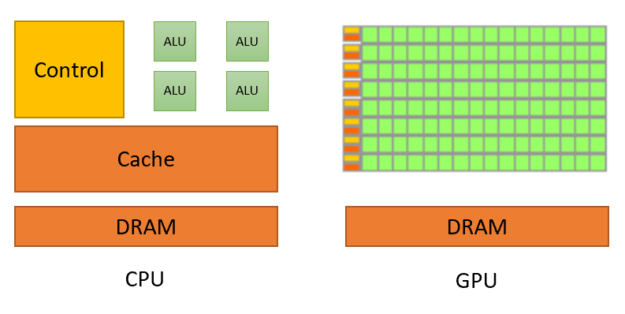
\includegraphics[width=\textwidth]{images/CPUvsGPU.png}
    % TODO: Pradeep Gupta, CUDA Refresher: Reviewing the Origins of GPU Computing, \url{CUDA Refresher: Reviewing the Origins of GPU Computing}, zuletzt aufgerufen am 17.06.2023

    Mit \enquote{ALU} als \enquote{algorithmic logic unit} oder \enquote{arithmetisch-logische Einheit}.

    Die CPU verfolgt das Konzept der geringen Latenz,
    wobei die GPU eine hohe Bandbreite anstrebt.
\end{defi}

\begin{defi}{GPU}{Programmausführung}
    \begin{enumerate}
        \item Kopieren der Eingabedaten vom CPU Speicher in den DRAM der GPU.
        \item Laden und Ausführen des Programms auf der GPU,
              wobei Caching für eine bessere Performance genutzt wird.
        \item Kopieren der Ergebnisse vom DRAM der GPU zurück in den CPU Speicher.
    \end{enumerate}
\end{defi}

\begin{defi}{Field Programmable Gate Array (FPGA)}
    \begin{itemize}
        \item Integrierter Schaltkreis, der vom Anwender selbst (anwendungsspezifisch) konfiguriert werden kann.
        \item Enthält eine Vielzahl von Logikschaltungen wie AND, XOR (bis zu mehreren Millionen Gatter).
        \item Einzelne Komponenten können hierarchisch und beliebig miteinander verschaltet werden.
        \item Logikblöcke enthalten in der Regel Speicher-Blöcke (z.B. Flip-Flops).
        \item Können je nach Bauart mehrfach oder nur einmal programmiert werden (Schmelzbrücken).
    \end{itemize}
\end{defi}

\begin{defi}[Field Programmable Gate Array (FPGA)]{Anwendungen}
    \begin{itemize}
        \item Es existiert eine Hardware Description Language (HDL) zur Konfiguration eines FPGAs, wobei Tools wie z. B. HDL Coder von MathWorks verfügbar sind.
        \item Ermöglichen effizientes Lösen komplexer und sehr spezifischer Aufgaben.
        \item Können genutzt werden, um Chip-Design (ASIC) und Funktionalität vorab zu testen, bevor die implementierte Logik als Chip produziert wird.
        \item Eignen sich ebenfalls als Beschleuniger, z.B. in Kombination mit einer Host-CPU.
        \item Schnelle Anbindung über QPI (QuickPath Interconnect, Intel) oder über PCIe.
    \end{itemize}
\end{defi}

\subsection{Aufgaben}

\begin{aufgabe}{Vektorprozessoren}
    Welche Eigenschaften müssen die Programmiersprache bzw. der Compiler haben um Vektorprozessoren nutzen zu können?
    \tcblower
    Die Programmiersprache muss Konstrukte zur Beschreibung der Vektoroperationen enthalten
    \underline{oder} der Compiler muss automatisch Programmteile als vektorisierbar erkennen.
\end{aufgabe}

\begin{aufgabe}{Parallelität}
    Erklären Sie den Unterschied zwischen ILP und DLP.
    \tcblower
    \begin{itemize}
        \item \emph{ILP (Instruction-Level Parallelism)} bezieht sich auf die Fähigkeit eines Prozessors,
              mehrere Anweisungen gleichzeitig auszuführen,
              indem er Anweisungen analysiert und versucht,
              Anweisungen zu finden,
              die unabhängig voneinander ausgeführt werden können.
              Der Prozessor kann dann diese Anweisungen parallel ausführen,
              um die Geschwindigkeit der Ausführung zu erhöhen.
        \item \emph{DLP (Data-Level Parallelism)} hingegen bezieht sich auf die Fähigkeit eines Prozessors,
              mehrere Datenströme parallel zu verarbeiten.
              Ein Beispiel für DLP ist die Verwendung von Vektorprozessoren,
              die in der Lage sind,
              mehrere Elemente eines Vektors gleichzeitig zu verarbeiten.
    \end{itemize}
\end{aufgabe}

\begin{aufgabe}{Vektorpipeline}
    Durch welche 3 Architekturkonzepte lässt sich die Datenverarbeitung mittels Vektorpipeline beschleunigen ?
    \tcblower
    \begin{itemize}
        \item Vektor-Pipleline Chaining
        \item Load/Store parallel zur Data Pipeline
        \item Load/Store Chaining
    \end{itemize}
\end{aufgabe}

\begin{aufgabe}[Pipelining]{ILP}
    Bei RISC-Prozessoren mit Pipelining ist eine Überlappung der Befehle bei der Ausführung möglich.
    Welcher Effekt kann diese Überlappung verhindern?
    \tcblower
    Register-Naming-Hazard
\end{aufgabe}

\begin{aufgabe}[Vektorpipeline]{Memory-Zugriffe}
    Welcher Effekt tritt beim unmittelbar nacheinander erfolgenden Zugriff auf Speicheradressen derselben Memory-Bank auf?
    \tcblower
    Totzeit des Speichers
\end{aufgabe}

\begin{aufgabe}[Vektorpipeline]{Memory-Zugriffe}
    Durch welche zwei Varianten kann ein Stride beim Zugriff auf die Memory-Bänke erzeugt werden?
    \tcblower
    \begin{itemize}
        \item explizit, d.h. durch Angabe der Schrittweite beim Schleifendurchlauf
        \item implizit durch Anordnung der Array-Elemente im Memory,
              sowie die Reihenfolge des Zugriffs auf diese
    \end{itemize}
\end{aufgabe}

\begin{aufgabe}{MSA}
    Beschreiben Sie kurz den Vorteil der MSA im Hinblick auf Beschaffungskosten von Superrechnern.
    \tcblower
    \begin{itemize}
        \item Es können einzelne Module ersetzt und mit bestehender HW verknüpft werden,
              das heißt,
              es muss nicht der komplette Supercomputer erneuert werden
        \item einzelne Module können unterschiedliche finanziert werden,
              z.B. durch verschiedene Fördertöpfe (Bund, Land)
    \end{itemize}
\end{aufgabe}
\section{Quantencomputer}

\begin{defi}[Quantencomputer]{Qubit}
    \begin{itemize}
        \item Digitaler Computer: Bit, Zustände: 0 oder 1
        \item Quantencomputer: Quantum Bit = Qubit,
              $\text{Zustände: } \alpha|0\rangle + \beta|1\rangle,$
              wobei $|0\rangle$ und $|1\rangle$ Quantenzustände und
              $\alpha, \beta$ Komplexe Zahlen mit $|\alpha|^2 + |\beta|^2 = 1$ sind.
    \end{itemize}
\end{defi}

\begin{defi}[Quantencomputer]{Operationen}
    TODO: Sinnvolle Definition
\end{defi}

\begin{defi}[Quantencomputer]{Nutzung}
    TODO: Sinnvolle Definition
\end{defi}

\begin{defi}[Quantencomputer]{Typische Programme}
    \begin{itemize}
        \item Shor: Faktorisierung in Primzahlen
              \begin{itemize}
                  \item \underline{Wichtig für:} Verschlüsselung / Kryptographie und andere sicherheitsrelevante Bereiche
                  \item \underline{Problem:} Für $n=p\cdot q$ finde Primfaktor $p$
                        (digitaler Computer: praktisch unmöglich ab 1024-bit)
                  \item \underline{Speedup durch Quantencomputer:} exponentiell
                  \item \underline{Warum:} Quantenparallelismus $|00\ldots00\rangle+$ $|00\ldots01\rangle+$ $|00\ldots10\rangle+$ $\ldots+$ $|11\ldots11\rangle$
              \end{itemize}
        \item Grover: Suche in Datenbanken
              \begin{itemize}
                  \item Problem: In $m$ Elementen $x_1, \ldots, x_m$ finde $x$ (digitaler Computer: $O(m)$)
                  \item Speedup durch Quantencomputer: quadratisch $O(\sqrt{m})$
              \end{itemize}
        \item Prinzipiell alle digitalen Algorithmen, aber nicht unbedingt schneller! $\to$ Beispiel: 2-bit Addition
    \end{itemize}
\end{defi}

\begin{defi}[Quantencomputer]{D-WAVE QUANTENANNEALER}
    Löst spezielles Optimierungsproblem \enquote{QUBO} schnell und effizient:
    \begin{align*}
        \min\limits_{q_i = 0,1}\left(\sum\limits_i a_i q_i + \sum\limits_{i<j} b_{ij} q_i q_j\right)
    \end{align*}
\end{defi}

\begin{bonus}[Quantencomputer]{Zusammenfassung}
    \begin{itemize}
        \item Quantencomputer = Idee aus Quantentheorie
        \item Kleinste Recheneinheit: 1 \hyperlink{defi:Qubit}{Qubit}
        \item Messung von \hyperlink{defi:Qubit}{Qubit} liefert Bit 0 oder 1
        \item Program = Schaltung aus Quantengattern
        \item Besondere Form: D-Wave Quantenannealer
        \item Werden digitale Computer durch Quantencomputer ersetzt? Nein!
        \item Nutzermodell: Programme schicken spezielle Teilprobleme an Quantencomputer
        \item Relevant für z. B. Faktorisierung, Suche in Datenbanken, Optimierung, \ldots
    \end{itemize}
\end{bonus}

\begin{jsc}{JUNIQ - Jülicher Nutzer-Infrastruktur für Quantencomputing}
    Das Ziel ist die Bereitstellung von \ldots
    \begin{itemize}[\ldots]
        \item Quantencomputer-Simulatoren (JUQCS, Atos QLM-30) über Cloud-Zugriff
        \item Zugängen zu verfügbaren Systemen für Anwender aus Wissenschaft und Industrie
              \begin{itemize}
                  \item Für diese sind Systeme mit verschiedenen technologischen Reifegraden (QTRL) verfügbar
                  \item Benutzer können erstmals das bevorzugte System auf einer QTRL-Rampe wählen:
                        \begin{itemize}
                            \item Zugriff auf aufkommende experimentelle Systeme
                            \item Zugriff auf Multi-Qubit-Systeme für Quantencomputing ohne Fehlerkorrektur (IBM, Google, Rigetti)
                            \item Hosting und Betrieb eines Systems für Quantenannealing (D-Wave Systems)
                        \end{itemize}
              \end{itemize}
        \item hochkarätiger Anwenderunterstützung in allen Aspekten der HPC- und Quantencomputer-Nutzung
              \begin{itemize}
                  \item Einrichtung eines unterstützenden Simulationslabors \enquote{Quantencomputing}
                  \item Forschungsteams für Quantenalgorithmen, Protokolle, Workflows und Software-Werkzeuge
              \end{itemize}
    \end{itemize}
\end{jsc}

\subsection{Aufgaben}

\begin{aufgabe}[Quantencomputer]{Qubits}
    Kreuzen Sie die richtigen Aussagen an.\\
    Qubits \ldots
    \begin{itemize}[label={\Square}]
        \item können drei Zustände annehmen.
        \item werden durch eine Messung in einen ihrer möglichen Zustände gezwungen.
        \item sind physhikalisch schwer zu erzeugen und ggf. instabil.
    \end{itemize}
    \tcblower
    Qubits \ldots
    \begin{itemize}[label={\Square}]
        \item können drei Zustände annehmen.
        \item [\XBox] werden durch eine Messung in einen ihrer möglichen Zustände gezwungen.
        \item [\XBox] sind physhikalisch schwer zu erzeugen und ggf. instabil.
    \end{itemize}
\end{aufgabe}

\begin{aufgabe}{Quantencomputer}
    Kreuzen Sie die richtigen Aussagen an.\\
    Quantencomputer \ldots
    \begin{itemize}[label={\Square}]
        \item können bestimmte Computeralgorithmen um ein Vielfaches schneller ausführen als herkömmliche Rechner.
        \item können herkömmliche Rechner komplett ersetzen.
        \item stellen eine Bedrohung für derzeitige Verschlüsselungsalgorithmen dar.
    \end{itemize}
    \tcblower
    Quantencomputer \ldots
    \begin{itemize}[label={\Square}]
        \item [\XBox] können bestimmte Computeralgorithmen um ein Vielfaches schneller ausführen als herkömmliche Rechner.
        \item können herkömmliche Rechner komplett ersetzen.
        \item [\XBox] stellen eine Bedrohung für derzeitige Verschlüsselungsalgorithmen dar.
    \end{itemize}
\end{aufgabe}

\printindex
\printindex[Beispiele]

%\printbibliography
\end{document}
